\chapter{Results and discussion}\label{results}

This chapter presents the statistical results from the \isi{eye tracking} recordings and the post-hoc questionnaires, and goes further in discussing them regarding the previously established hypotheses. The hypotheses on \isi{visual attention} were tested by analysing the eye movements of the 45~participants to determine whether integrated titles result in shorter \isi{reading time} (\isi{fixation duration} on the titles), more attention on the image than the \isi{title area}, and a \isi{gaze behaviour} more equivalent to the \isi{natural focus} points of the English native speakers. Another focus was the impact of the individual \isi{placement} on reaction times (time to \isi{first fixation}). In the following summary of the results, “OV” is used to describe the original version the English-speaking participants watched. The traditionally subtitled version is abbreviated to “TS” (traditional subtitles) and the version with integrated titles to “IT” (integrated titles).


\section{{Fixation-based data}}\label{sec:8.1}

Based on the pilot study, it was assumed that by individually adjusting the formatting of a title, its \isi{font} and \isi{placement}, the \isi{fixation} time per title would decrease compared to the traditional counterparts. These adjustments allow for faster processing (e.g. by creating a stronger contrast), and the \isi{placement} closer to the \isi{natural focus} motivates the audience to return to exploring the image faster.



The following statistical data is based on the eye movement recordings of the 45 participants (14 English natives and 31 German natives) of the three film versions (original, subtitled, integrated titles). The subtitled version was created with \textit{Subtitle Workshop} and the version with integrated titles was created in \textit{Premiere Pro}. The film version with the traditional subtitles included 132 subtitles and the version with the integrated titles included 152 titles (as dialogues, pauses, and hesitation were taken into account and corresponding titles split into several). Each scene containing a title received one AOI around the title and one AOI around the image (excluding the black frame around the film). Including \isi{film title} and \isi{prologue} texts, this resulted in 271 \isi{AOIs} for the TS condition and 312 \isi{AOIs} for the IT condition. These \isi{AOIs} were each drawn by hand and the timing adjusted to perfectly reflect the display duration of each title (between one and six seconds). Additionally, 23 clusters were created for ten scenes with titles. The corresponding heat maps, clusters, and \isi{gaze} plots were exported for each scene of each of the three conditions of the film containing text, amounting to 416 visualisations of eye movement data each. Based on the \isi{AOIs}, a number of measures could be extracted from the data and analysed based on the previously stated hypotheses. 


\subsection{Hypothesis 1 – Fixation duration}\label{sec:8.1.1}

\textit{“Fixation duration in the \isi{title area} is shorter for IT than for TS.”}

\bigskip

The first hypothesis states that the integrated titles have an effect on the \isi{fixation duration} on the title, i.e. \isi{fixation duration} will be shorter, reflecting an easier information extraction (\citealt{Jacob2003}:~585; \citealt{mccarthy2003}:~409; cf. \citealt{Fitts1950}; see Chapter~6.4). The reading times of the participants were calculated by measuring the durations of the fixations and saccades in the area of the title – expressed in the average total \isi{visit duration}. The \isi{reading time} for each subtitle by each of the 15 German participants in the second group (in the following referred to as “TS participants”) and for each title by each of the 16 German participants in the third group (the “IT participants”) was recorded. As the Shapiro-Wilk test showed a deviation from a normal distribution, the two data sets – the reading times of the TS participants and the IT participants – were compared using the Wilcoxon test: W = 1675877, p < 0.001. As the error probability p is clearly below the tolerable 5\,\% (0.05), there is a significant difference between the two data sets. The following mean (m) and standard deviation (sd) values were calculated:
\bigskip

\begin{tabular}[t]{lr} 
m(total\_visit\_duration\_iT) = 1.570~s & m(total\_visit\_duration\_tU) = 1.835~s\\
sd(total\_visit\_duration\_iT) = 1.069~s & sd(total\_visit\_duration\_tU) = 1.159~s\\
\end{tabular}

\bigskip
The difference between the two mean values is about 265~ms – a significant reduction of 14.4\,\% of the \isi{reading time} for integrated titles compared to the average \isi{reading time} for traditional subtitles (see \figref{fig:FIG58chart4}). Therefore, the participants seemed to have less \isi{difficulty extracting information} from the integrated titles, possibly due to the more considerate \isi{placement} and proximity to the \isi{main focus} points.


\begin{figure}
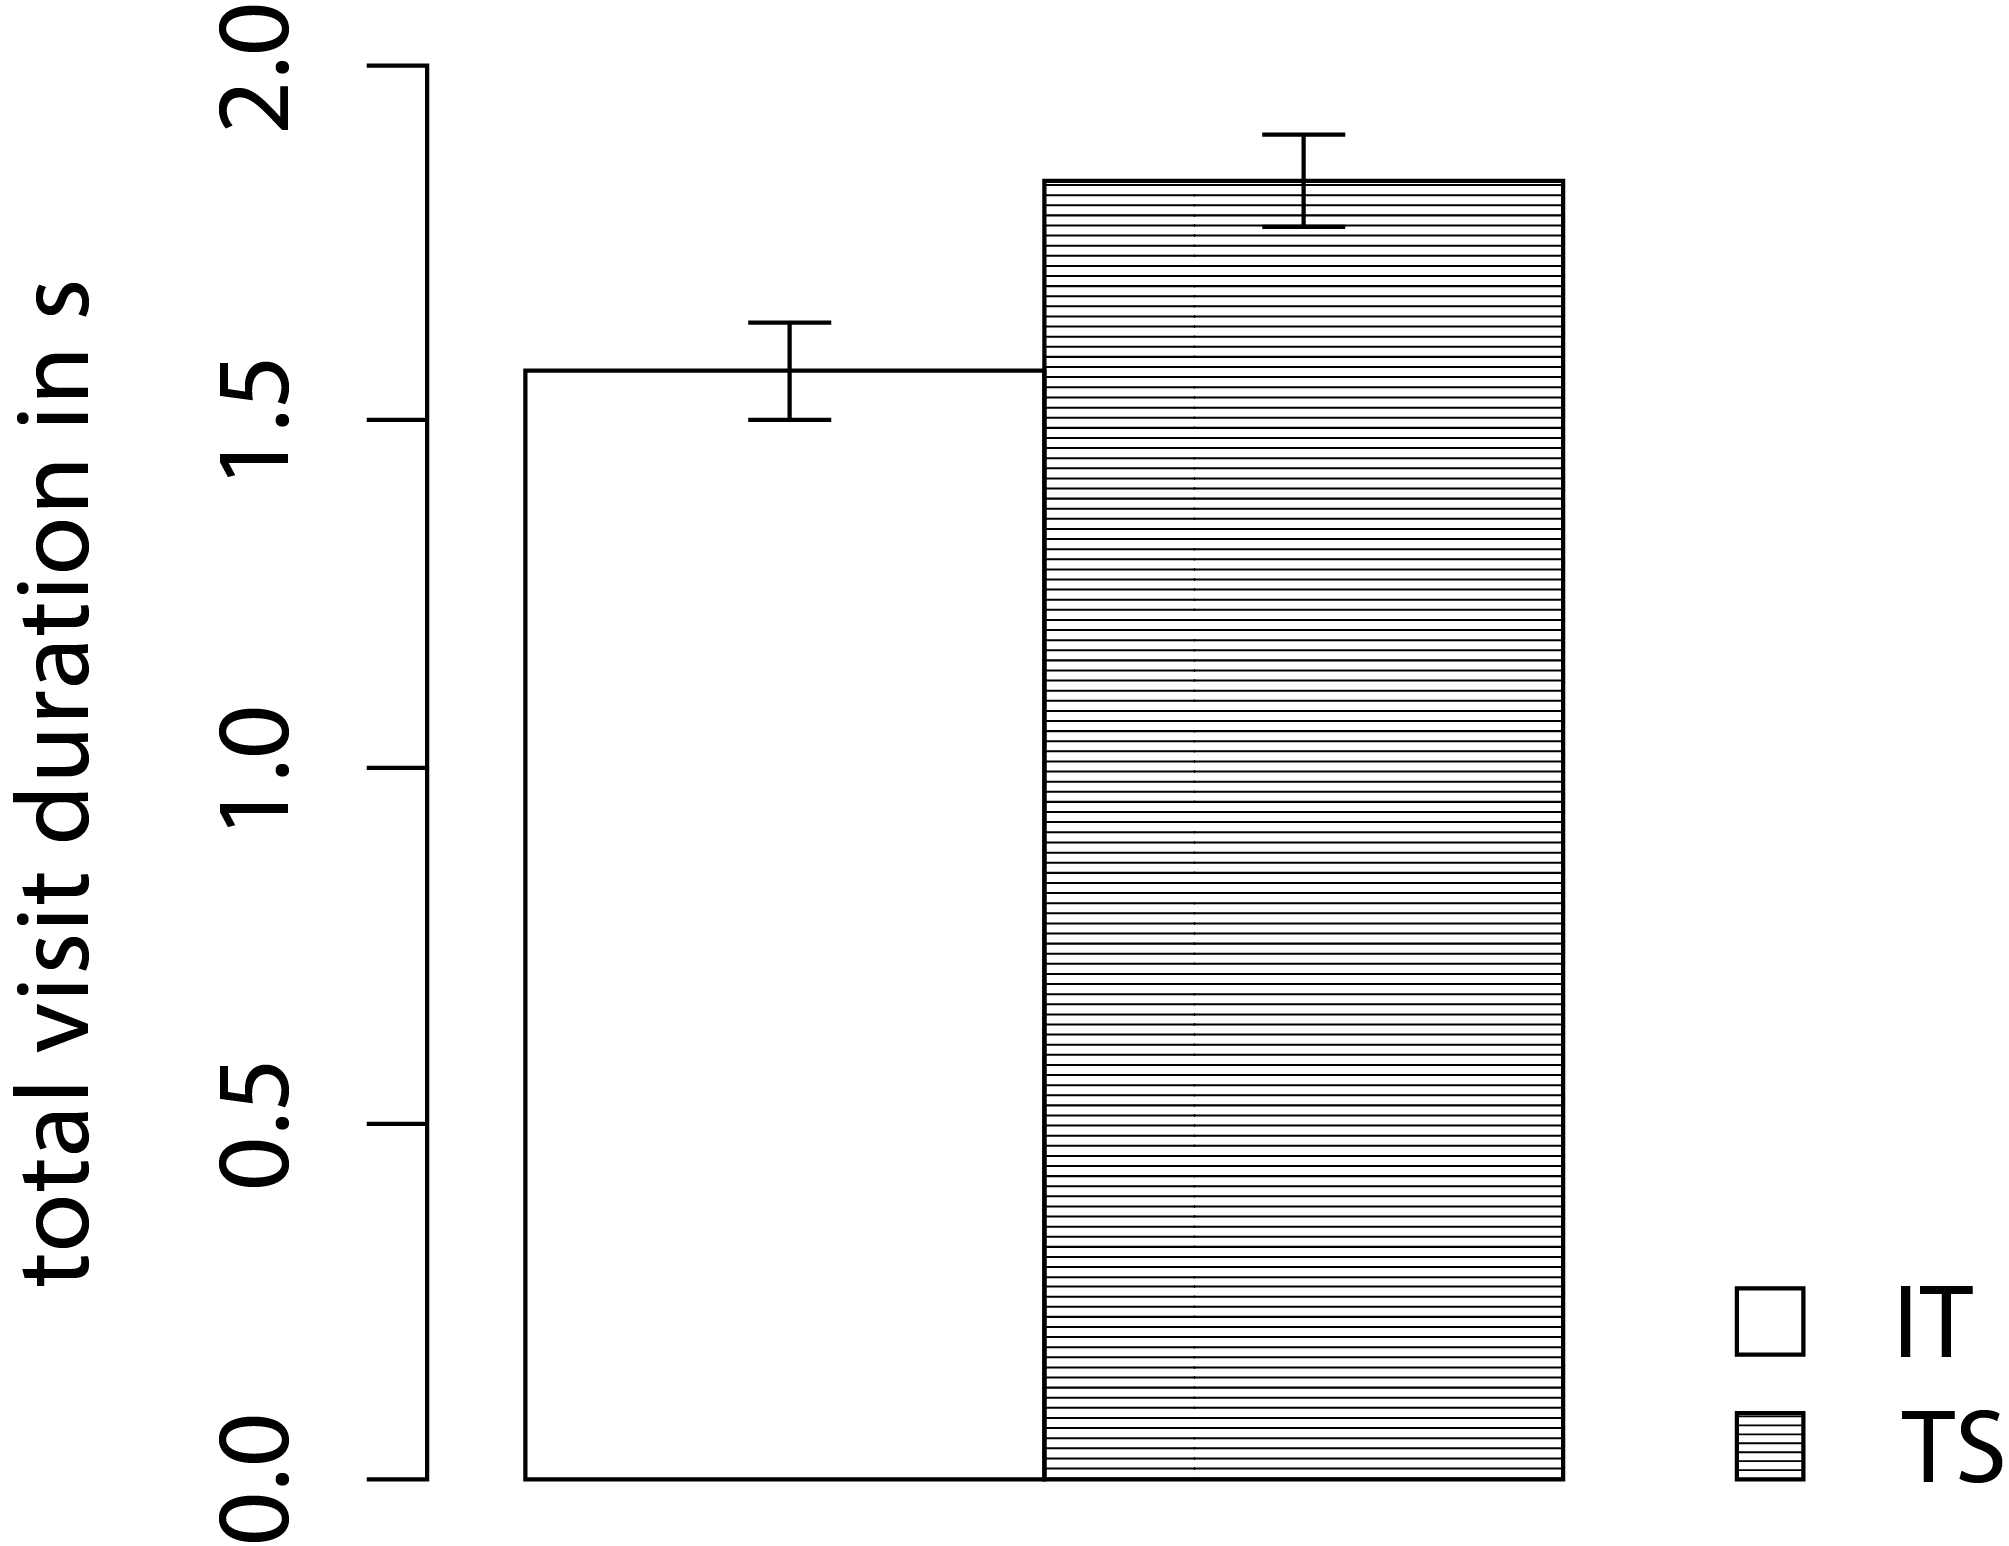
\includegraphics[width=0.7\textwidth]{figures/FIG58chart4.png}
\caption{Comparison of the average total visit duration (s) of the IT and TS participants}
\label{fig:FIG58chart4}
\end{figure}

To give an impression of the underlying data, the mean values of the TVD (total visit duration) per title are illustrated in \figref{fig:FIG59chart5} for the first 30 subtitles and titles.

\begin{figure}
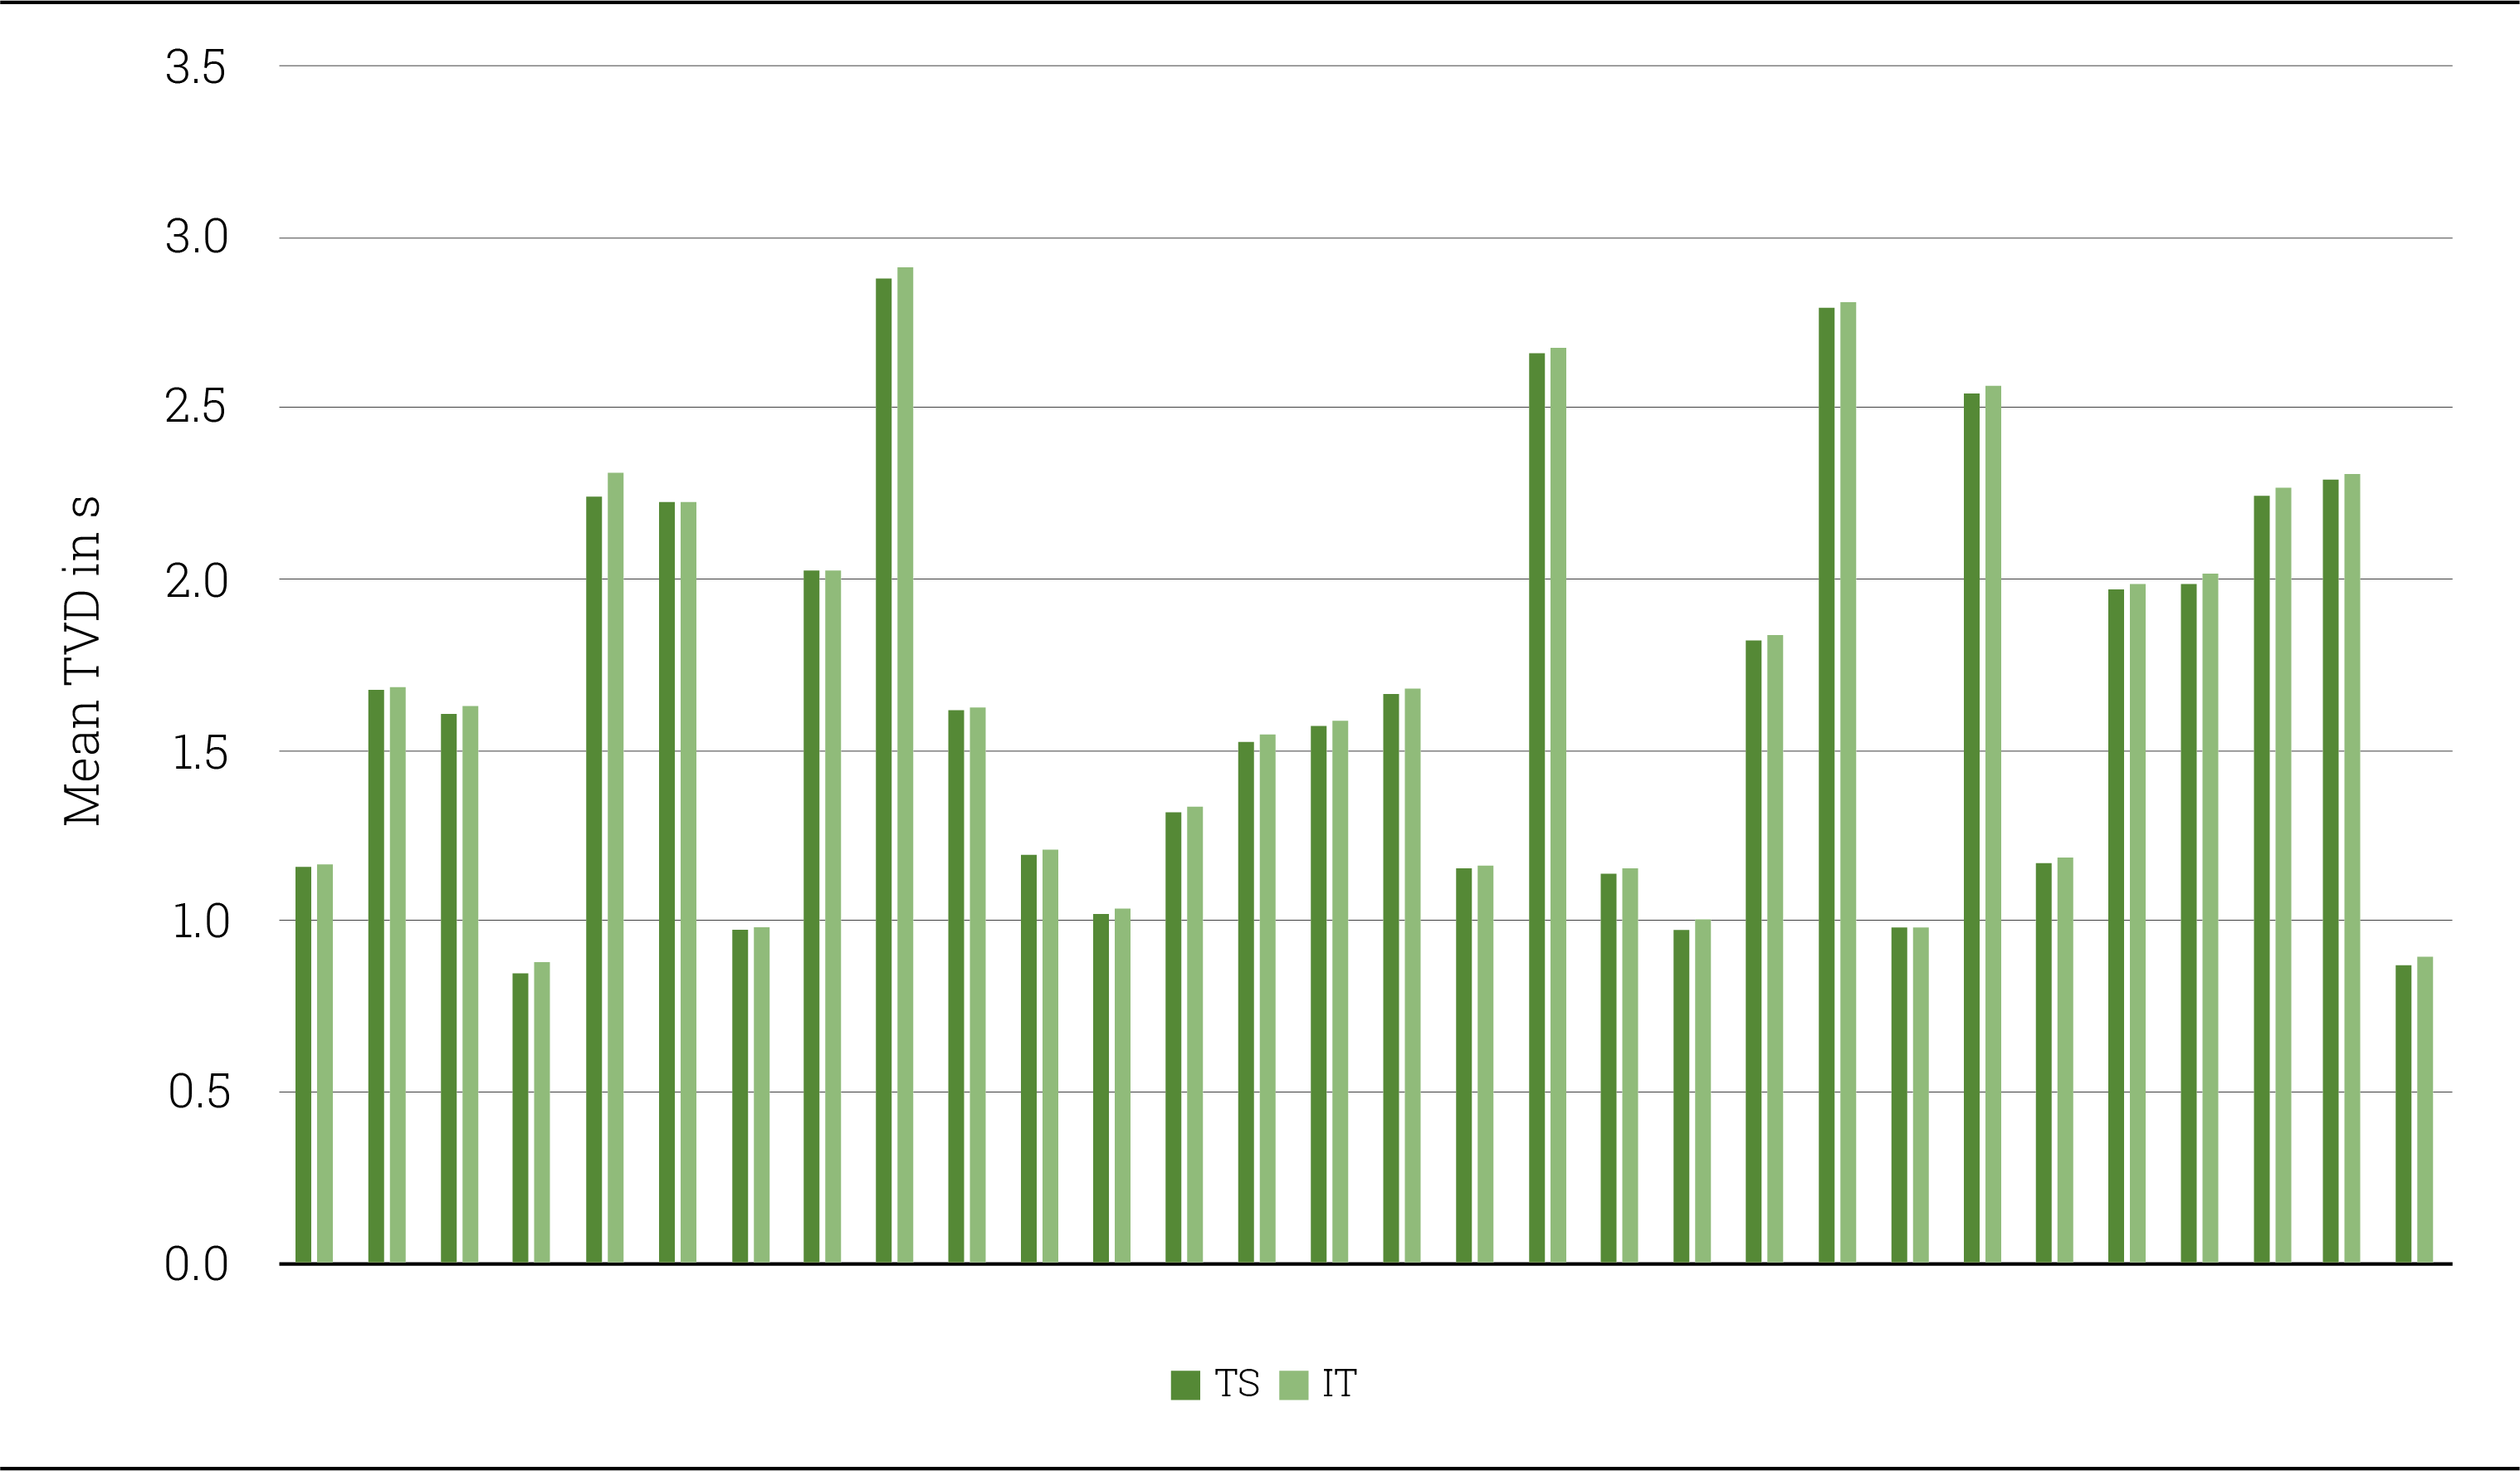
\includegraphics[width=\textwidth]{figures/FIG59chart5.png}
\caption{Sample of the mean TVD per title}
\label{fig:FIG59chart5}
\end{figure}

\subsection{Hypothesis 2 – Split attention}\label{sec:8.1.2}

\textit{“IT participants spend more time fixating (exploring) the image than fixating (reading) the titles, experiencing a \isi{positive split attention}.”}
\bigskip

As visible from the results concerning the first hypothesis, the IT participants spent less time focusing the titles compared to the TS participants. Based on this assumption, the second hypothesis states that the participants with integrated titles spend more time exploring the image than looking at the title. This measurement of \isi{visual attention} was defined as \isi{split attention} between image and \isi{title area}. To test this hypothesis, the average total \isi{visit duration} (TVD) of both the entire image and the \isi{title area} during the stimulus, meaning the time between the title fading in and out, was measured. For all four data sets (TVD of the image TS/IT and TVD of the \isi{title area} TS/IT), the Shapiro-Wilk test showed a deviation from normal data distribution. The Wilcoxon test then showed significant differences between the corresponding data sets:
\bigskip

\eabox{
\small
\begin{tabular}[t]{lr} 
wilcox.test(TVD\_IT\_IMAGE, TVD\_IT\_TITLE): & W = 4400522, p < 0.001\\
wilcox.test(TVD\_TS\_IMAGE, TVD\_TS\_TITLE): & W = 2769346, p < 0.001\\
wilcox.test(TVD\_TS\_IMAGE, TVD\_IT\_IMAGE): & W = 2616334, p < 0.001\\
wilcox.test(TVD\_TS\_TITLE, TVD\_IT\_TITLE): & W = 2217703, p < 0.001\\
\end{tabular}

\bigskip

\begin{tabular}[t]{lr} 
m(TVD\_IT\_IMAGE) = 3.306~s & m(TVD\_IT\_TITLE) = 1.570~s\\
m(TVD\_TS\_IMAGE) = 3.555~s\footnotemark{} & m(TVD\_TS\_TITLE) = 1.835~s\\
\end{tabular}
}

\footnotetext{The duration of the average TVD on the image differs between the two conditions because some participants would leave the image AOI, e.g. looking away from the screen or the video that was surrounded by a black frame.}

\bigskip
The results show that on average the TS participants focused on the \isi{subtitle area} for 51.6\,\% of the \isi{title display} duration, on average 1.835~s of 3.555~s. For integrated titles, the participants focused on the \isi{title area} for around 47.5\,\% of the time (on average 1.57~s of 3.306~s; see \figref{fig:FIG60chart6}).

\begin{figure}
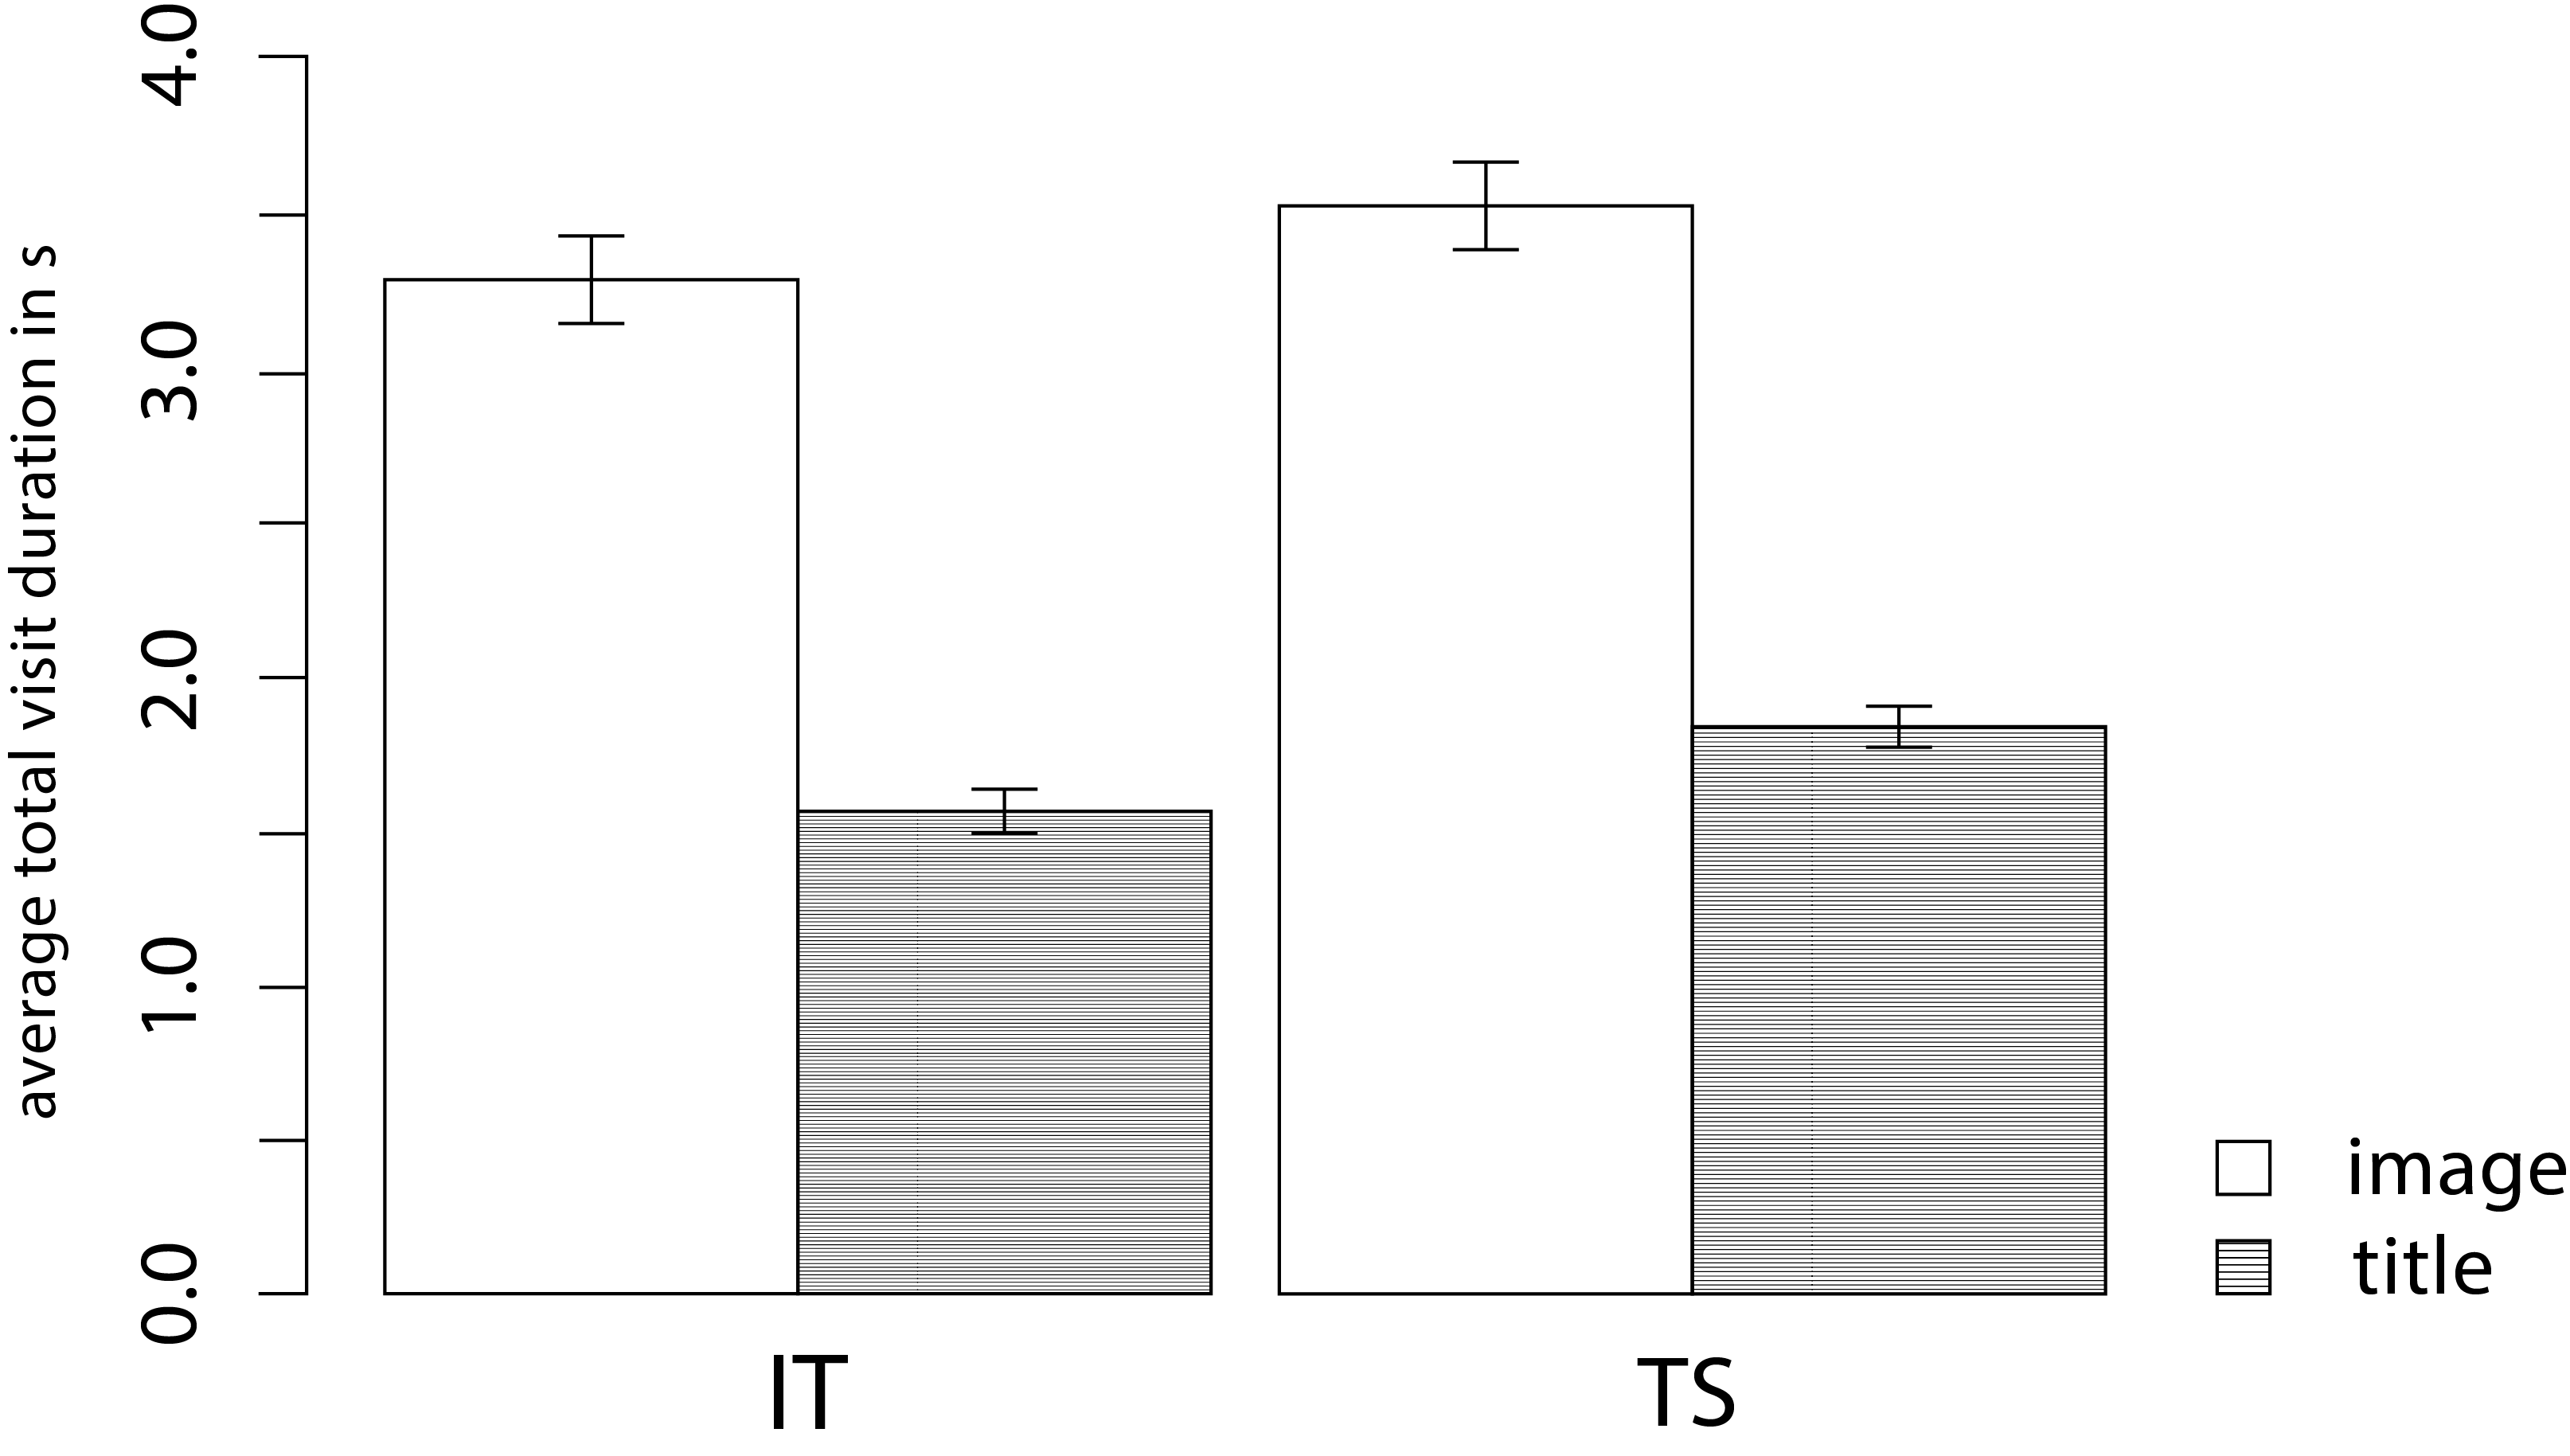
\includegraphics[width=0.8\textwidth]{figures/FIG60chart6.png}
\caption{Comparison of split attention in IT and TS participants}
\label{fig:FIG60chart6}
\end{figure}

This indicates that integrated titles motivate the audience to return to the actual \isi{focal point} in the image faster and spend more time exploring the image while the title is visible. This is also supported by the low number of participants who fixated the \isi{title area} before the title was faded in (see the discussion of the fourth hypothesis in \sectref{sec:8.1.4}).

\subsection{Hypothesis 3 – Natural focus}\label{sec:8.1.3}
\textit{“The focus of the IT participants resembles the \isi{natural focus} of the native viewers considerably more than the focus of the TS participants.”}
\bigskip

The third hypothesis states that IT participants are more likely to display a more \isi{natural gaze behaviour}, based on the \isi{natural focus} points of the English participants, than the TS participants. The hypothesis was tested by means of a random sample of ten titles and the therein defined 23~relevant areas of attention. These areas were defined through automatically generated cluster area and the \isi{gaze behaviour} of the TS and IT participants was compared to that of the 14~English native speakers. The automatically generated clusters, areas of accumulated fixations created by \textit{Tobii Studio}, were defined as the \isi{natural focus} points if more than 50\,\% of the participants fixated it at least once (see \figref{fig:FIG61}).

\begin{figure}
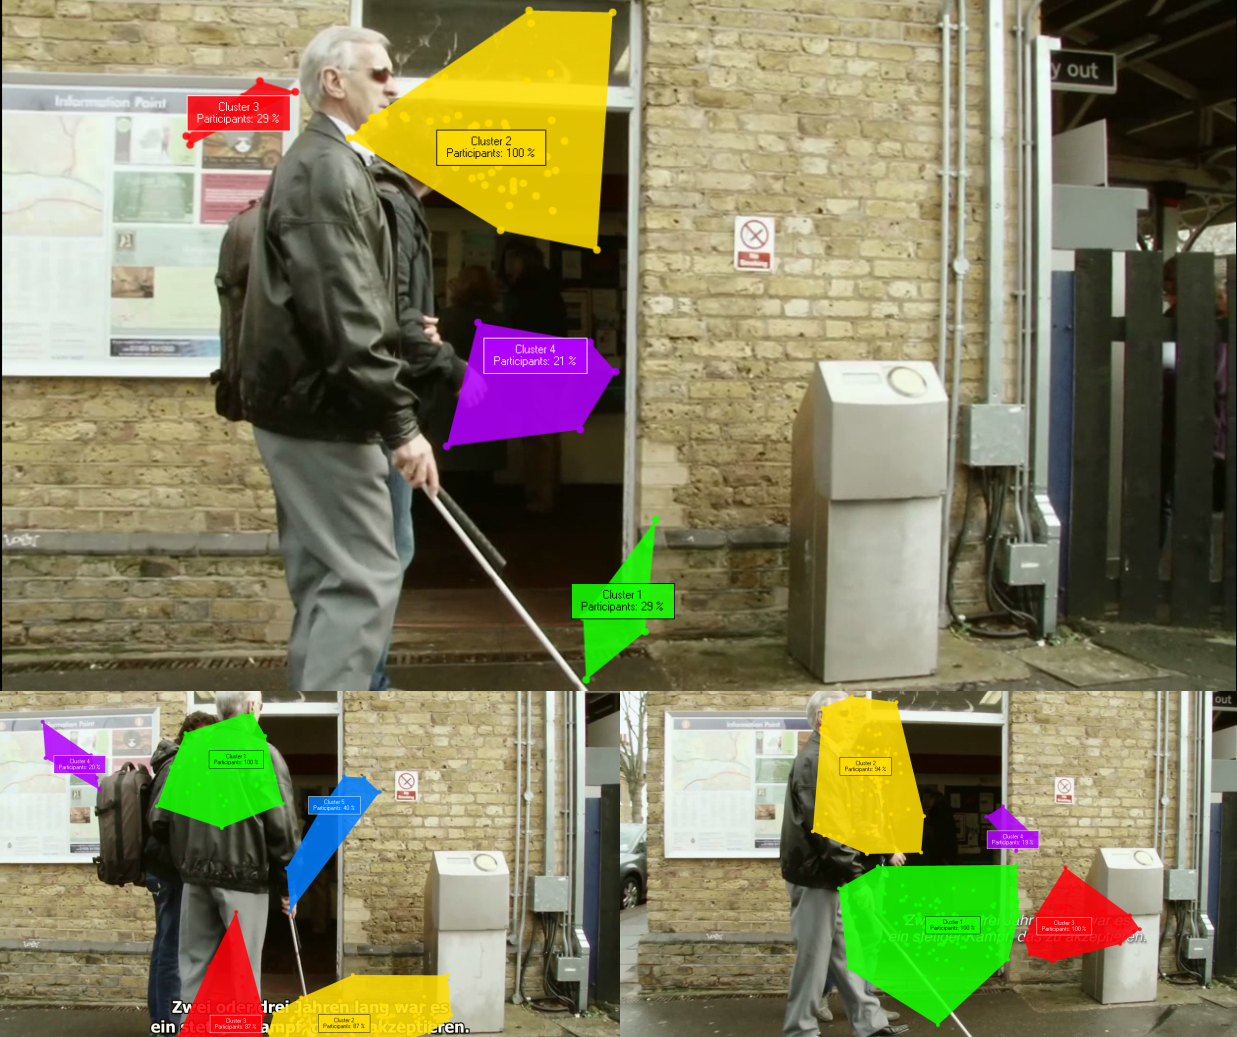
\includegraphics[width=\textwidth]{figures/FIG61.jpg}
\caption{Comparison of the automatically created clusters OV/TS/IT (\textit{Joining the Dots}, UK 2012)}
\label{fig:FIG61}
\end{figure}

These clusters were created for ten random scenes\footnote{Excluding scenes in which a subtitle (TS) was divided into several titles (IT) and scenes that consisted exclusively of a title in front of a black background. The first few scenes only consisted of the \isi{film title} and \isi{prologue} and were therefore skipped.} and considered only when they were fixated by at least half of the corresponding participant group. Four clusters were not evaluated as they could not be interpreted clearly (marked in red in the following table) while 23~clusters were evaluated (see \tabref{tab:TAB14}). During this sample, the \isi{natural focus} points – the clusters which at least 50\,\% of participants viewed – were fixated by an average 87.87\,\% of the OV~participants. Clusters at the same spot or very close were fixated by an average 75.3\,\% of the TS~participants and 83.3\,\% of the IT~participants. Thus, the integrated titles increased the mean number of participants that fixated the \isi{natural focus} points of the English natives by 10.6\,\%. Additionally, the sample showed that, on average, 88.1\,\% of the TS participants fixated the subtitle while about 98.2\,\% of the IT participants fixated the integrated titles – an increase of 11.5\,\%. 

\begin{table}
\begin{tabularx}{\textwidth}{lQrrr}
\lsptoprule   Cluster &  Fixated Element / Area &  OV &  TS &  IT\\
\midrule
014--1 & Finger tips on white cane & 100\,\% & 93\,\% & 88\,\%\\
014--2 & Sub(title) & \textit{NA}\footnote{As the original version does not include any subtitles, there are no reportable values for the OV version.} & 80\,\% & 100\,\%\\
024--1 & Heads & 100\,\% & 100\,\% & 94\,\%\\
024--2 & Sub(title) & \itshape NA & 87\,\% & 100\,\%\\
034--1 & Eye/face left & 100\,\% & 73\,\% & 75\,\%\\
034--2 & Eye right & 71\,\% & \itshape unclear & 38\,\%\\
034--3 & Sub(title) & \itshape NA & 100\,\% & 100\,\%\\
044--1 & Head left & 100\,\% & 80\,\% & 94\,\%\\
044--2 & Heads right & 64\,\% & 93\,\% & 69\,\%\\
044--3 & Sub(title) & \itshape NA & 100\,\% & 100\,\%\\
054--1 & Face & 100\,\% & 80\,\% & 100\,\%\\
054--2 & Sub(title) & \itshape NA & 80\,\% & 100\,\%\\
064--1 & Eyes & 93\,\% & 87\,\% & 100\,\%\\
064--2 & Mouth & 50\,\% & 53\,\% & 100\,\%\\
064--3 & Sub(title) & \itshape NA & 80\,\% & 94\,\%\\
076--1 & Face & 100\,\% & 87\,\% & 100\,\%\\
076--2 & Sub(title) & \itshape NA & 87\,\% & 100\,\%\\
084--1 & Stage right & 100\,\% & \itshape unclear & 56\,\%\\
084--2 & Stage left & 79\,\% & \itshape unclear & \itshape unclear\\
084--3 & Sub(title) & \itshape NA & 87\,\% & 100\,\%\\
094--1 & Hands & 100\,\% & 93\,\% & 69\,\%\\
094--2 & Face right & 100\,\% & 53\,\% & 44\,\%\\
094--3 & Sub(title) & \itshape NA & 87\,\% & 94\,\%\\
104--1 & Trevor’s face & 64\,\% & 47\,\% & 75\,\%\\
104--2 & Sheep head & 79\,\% & 47\,\% & \itshape unclear\\
104--3 & Hands & 71\,\% & 40\,\% & 75\,\%\\
104--4 & Sub(title) & \itshape NA & 93\,\% & 94\,\%\\
\lspbottomrule
\end{tabularx}
\caption{Overview of the fixation percentages of the analysed cluster areas}
\label{tab:TAB14}
\end{table}

At the first glance, however, five elements show a higher \isi{fixation} percentage of the TS participants than the IT participants. These five entries (014--1, 024--1, 044--2, 094--1, and 094--2) take place in four scenes. In Scene~014, the reason is easy to find: The subtitle is much closer to the relevant element and the integrated titled, even though being placed with more consideration of the \isi{image composition}, is just too far away (see \figref{fig:FIG62fig56}).
\clearpage 

\begin{figure}
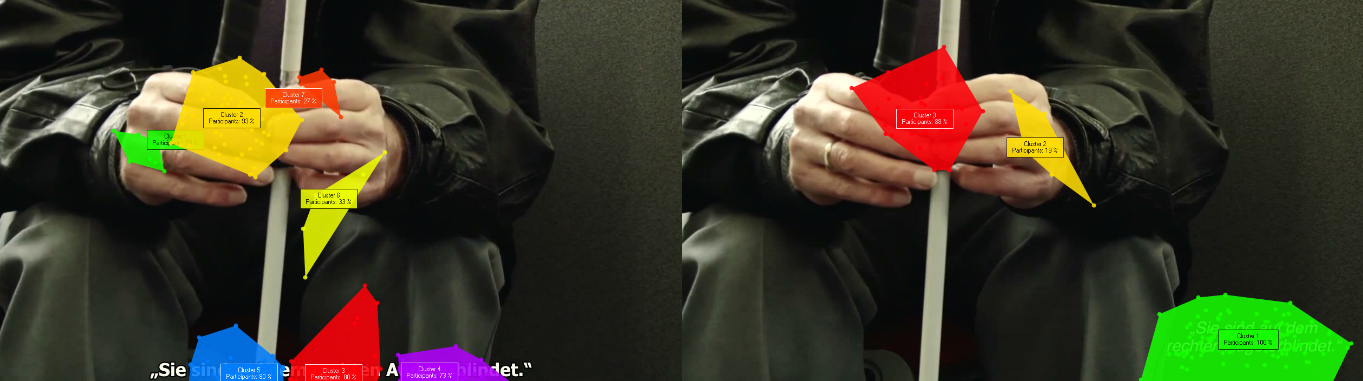
\includegraphics[width=\textwidth]{figures/FIG62fig56.jpg}
\caption{Comparison of the automatic clusters in Scene 014 (TS on the left, IT on the right)}
\label{fig:FIG62fig56}
\end{figure}

Despite this suboptimal \isi{placement} of the integrated title, the average combined attention percentage of title and element is still higher for the IT participants (94\,\% for IT and 86.5\,\% for TS). The same goes for the \isi{combined average attention} percentage in Scene~024 (97\,\% for IT and 93.5\,\% for TS). For Scene~044, the reason for the lower attention percentage is quite elusive (81.5\,\% \isi{combined average attention} for all three elements for IT and 86.5\,\% for TS) as the titles are in almost identical positions. Based on the low amount of integrated titles and subtitles in general placed in the top area of the image (see \chapref{placement}), the differences in Scene~094 could have been caused by the position being too unexpected for the viewers (see \figref{fig:FIG63fig57}).

\begin{figure}
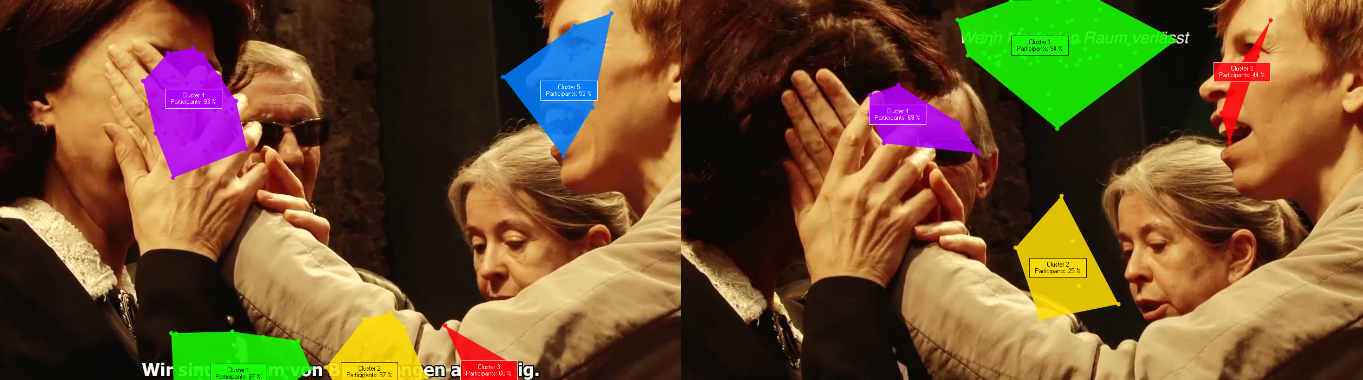
\includegraphics[width=\textwidth]{figures/FIG63fig57.jpg}
\caption{Comparison of the automatic clusters in Scene 094 (TS on the left, IT on the right)}
\label{fig:FIG63fig57}
\end{figure}

This shows that there is still plenty of room for improvement concerning the \isi{placement} of integrated titles and further research could, for example, look at the effects of horizontal and vertical displacement compared to the traditional subtitle position.

All in all, a higher percentage of the IT participants in this random sample focused both on the \isi{natural focus} points of the OV participants and the displayed titles. This indicates that integrated titles allow for a more \isi{natural focus} for the audience and at the same time seem to motivate the viewer to fixate a higher percentage of the titles and extract information both faster and more effectively.

\subsection{Hypothesis 4 – Reaction time}\label{sec:8.1.4}

\textit{“The \isi{reaction time} of the IT participants is higher than that of the TS participants.”}
\bigskip

The hypothesis of integrated titles increasing the \isi{reaction time} is based on the assumption that an audience that is used to subtitles has already learned to switch focus to the bottom area as soon as someone in the film starts speaking. For integrated titles, one can assume that the \isi{title area} is not focused until the fade-in effect initiates the eye movement (cf. “involuntary attention”, \citealt{prinzmetal2005}:~74). To test this hypothesis, \isi{AOIs} were defined for each subtitle and title. They allow measurements of the \isi{reaction time}, meaning the duration between when the title fades in and the \isi{first fixation} in the corresponding AOI (“time to \isi{first fixation}”, TFF). The data of the 15 TS and the 16 IT participants were compared and, as the Shapiro-Wilk test was significant for both data sets, the Wilcoxon test was applied: W = 2281026, p < 0.001. The \isi{reaction time} of the IT participants (74~ms) was on average 28.9\,\% higher (17~ms) than for the TS participants (57~ms, see \figref{fig:FIG64chart8}).

\begin{figure}
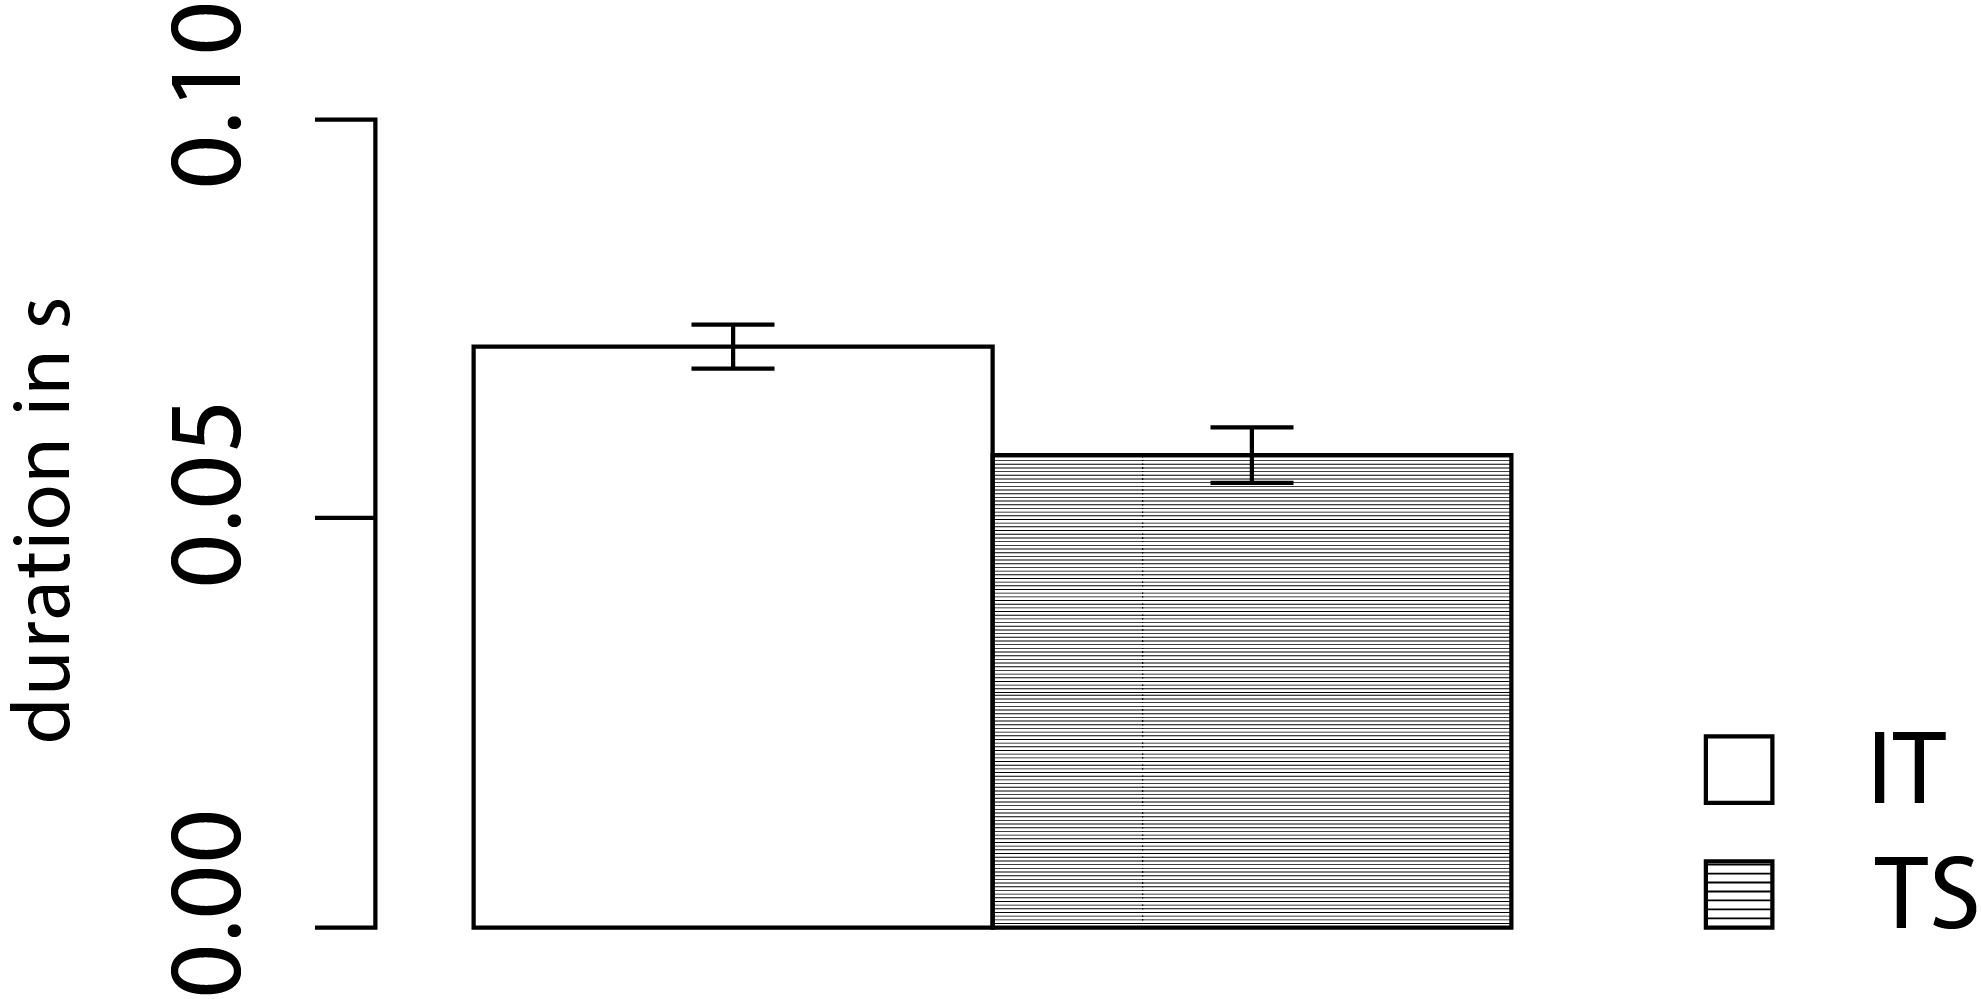
\includegraphics[width=0.7\textwidth]{figures/FIG64chart8.png}
\caption{Mean reaction time}
\label{fig:FIG64chart8}
\end{figure}

Due to the very short time frame in which the titles are visible, the difference in the TVD and \isi{split attention} seemed quite small. Therefore, the explorative behaviour right before the stimulus should be examined in addition to the reaction times. A \isi{reaction time} of 0 means that a participant had already focused on the area before the title was displayed. This value would be expected to only occur rarely, e.g. between consecutive titles containing long sentences.

\begin{figure}
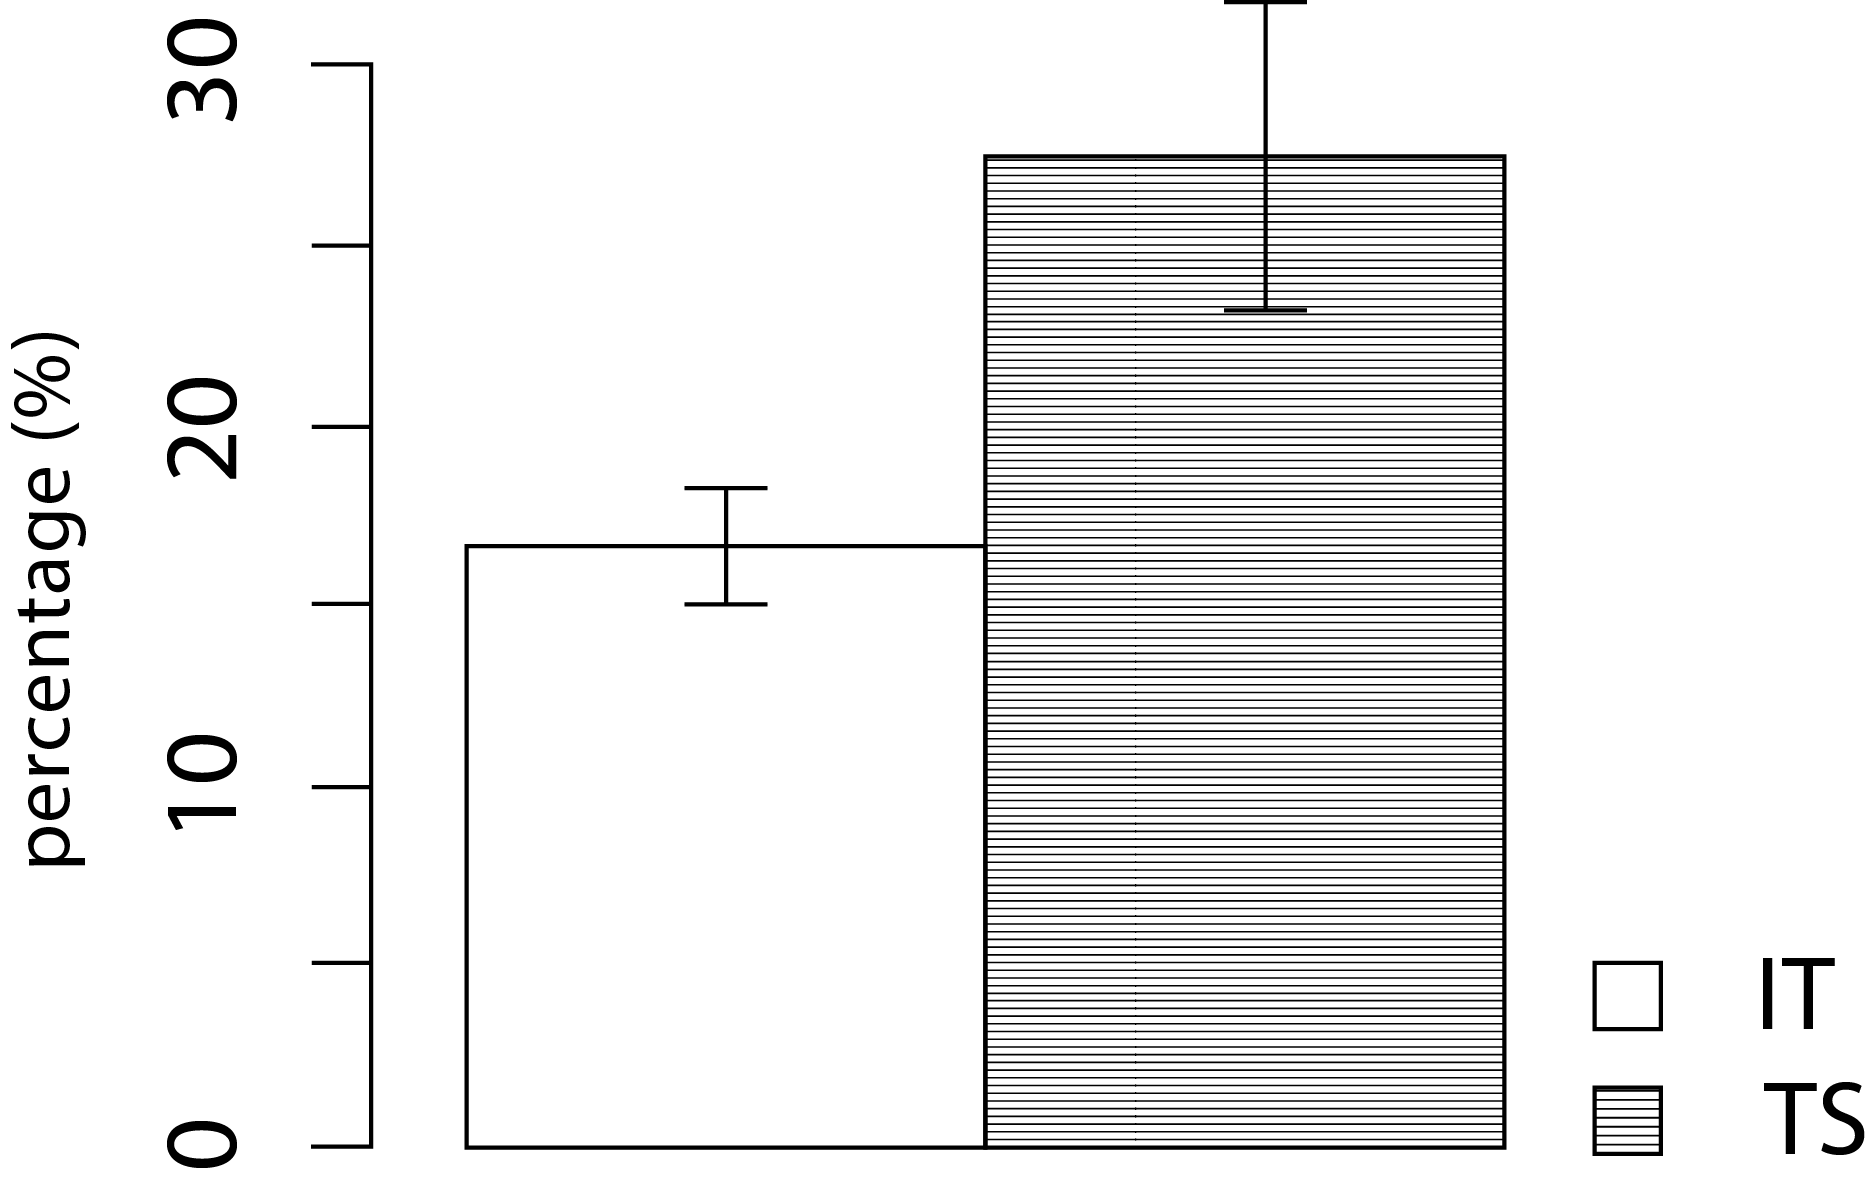
\includegraphics[width=0.7\textwidth]{figures/FIG65chart8.png}
\caption{Average percentage of 0 values of TS and IT participants in TFF}
\label{fig:FIG65chart8}
\end{figure}

\figref{fig:FIG65chart8} shows the average percentage of 0 values in the TFF per participant per group. For each IT participants, the value 0 occurred on average 23.1 times and 33.4 times for each TS participants; this corresponds to 16.5\,\% of all reaction times for the IT participants and about 27.5 \% for the TS participants. Therefore, the TS participants focused on the \isi{title area} before the stimulus significantly more often while the IT participants remained focused on the image for a longer time. Omitting the 0 values, the increase of the \isi{reaction time} was about 25.9\,\% (instead of 28.9\,\%) – from 69~ms for TS participants to 87~ms for the IT participants (see \figref{fig:FIG66chart9}).

\begin{figure}
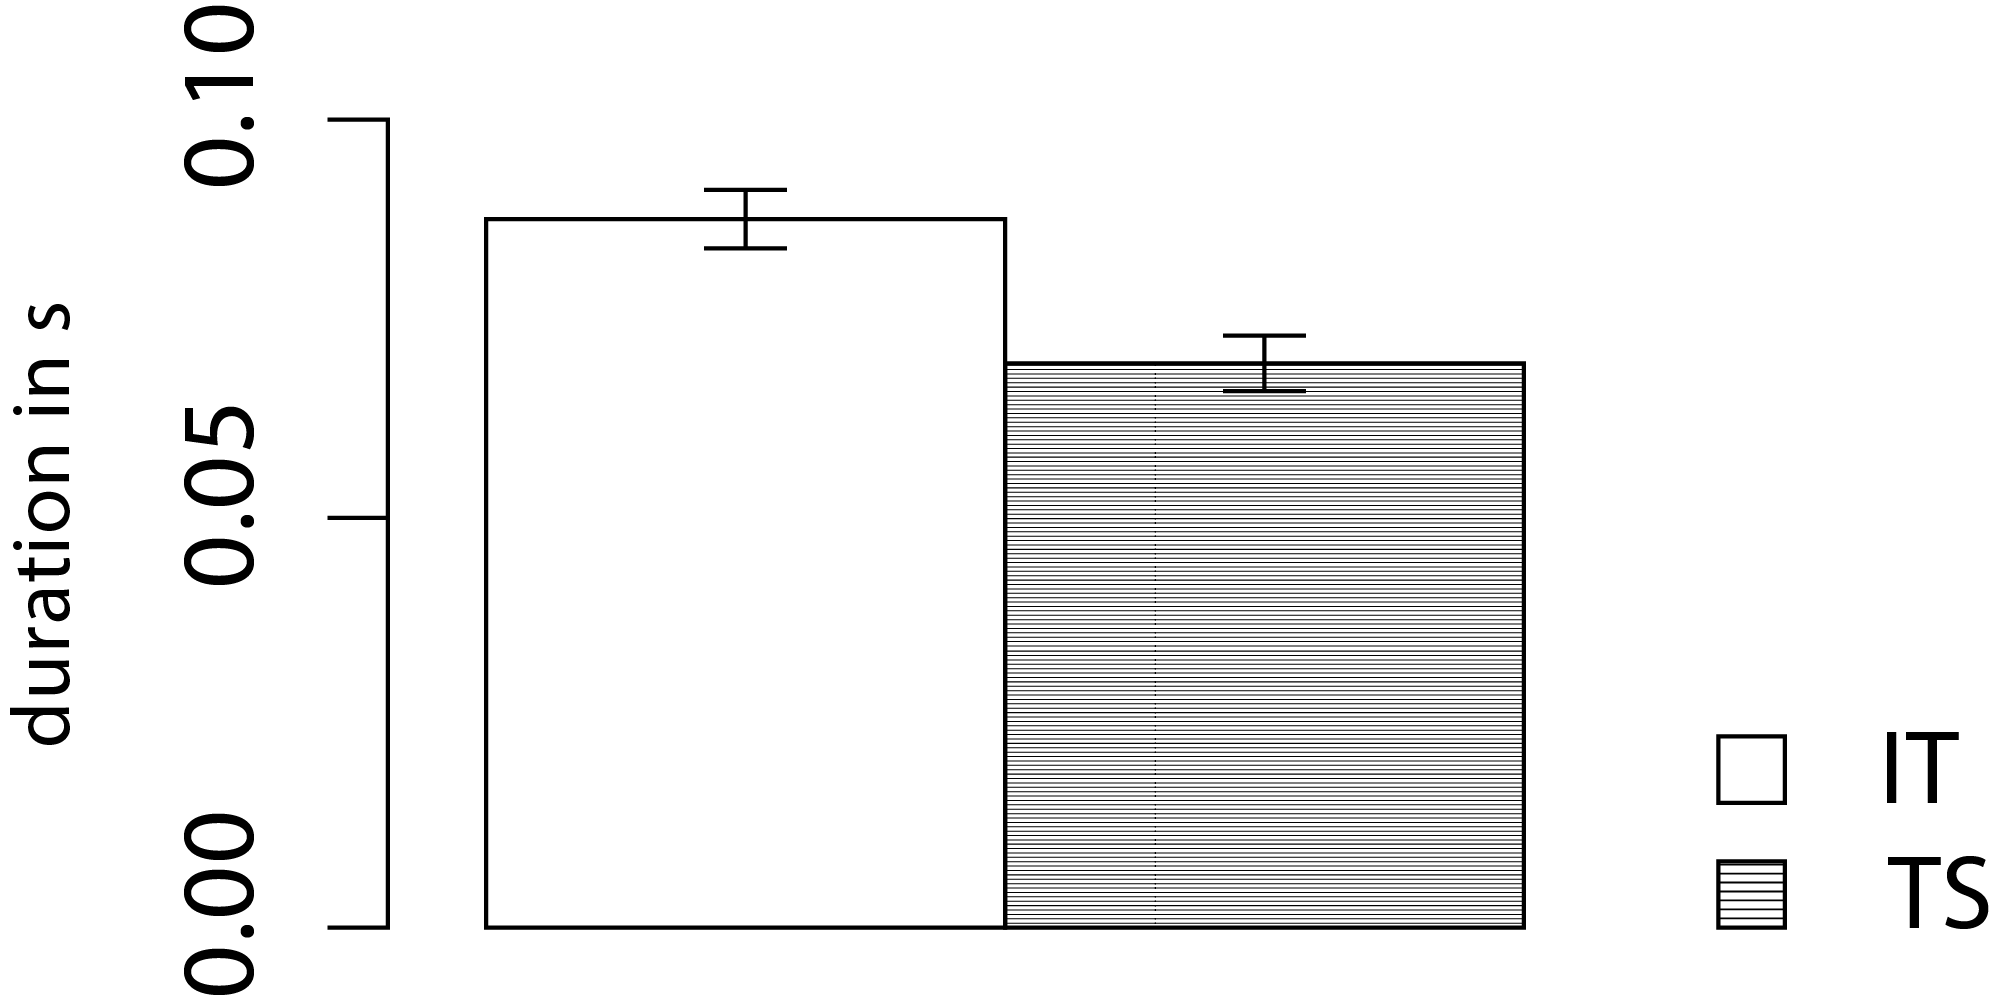
\includegraphics[width=0.7\textwidth]{figures/FIG66chart9.png}
\caption{Mean reaction time without the 0 values}
\label{fig:FIG66chart9}
\end{figure}

\newpage 
An increased \isi{reaction time}, however, cannot strictly be interpreted as a negative effect: While a shorter \isi{reaction time} might be associated with less cognitive load for the viewer or a higher level of stress, a longer \isi{reaction time} might also be synonymous with the longer \isi{image exploration} demonstrated by the IT participants or an overall more relaxed viewing.

\section{Questionnaire data – Hypotheses 5 and 6}\label{sec:8.2}

In addition to recording the eye movements and analysing the attention and reaction of the participants, a questionnaire on the \isi{aesthetic experience} was also part of the study. As eye movements cannot tell us very much about the subjective feelings of a participant, all participants with integrated titles were asked to rank several statements after watching \textit{Joining the Dots}.\footnote{The questionnaire was designed following the recommendations on \url{http://www.wpgs.de/content/blogcategory/87/355/} [2015--01--06, in German].}

The questionnaire was divided into a general part with statements on \isi{information intake} and a second part focusing on the \isi{aesthetic experience}. The participants could rank the statements on a scale from 1 (“agree strongly”) to 4 (“disagree strongly”), as illustrated in \figref{fig:FIG67fig58}:

\begin{figure}
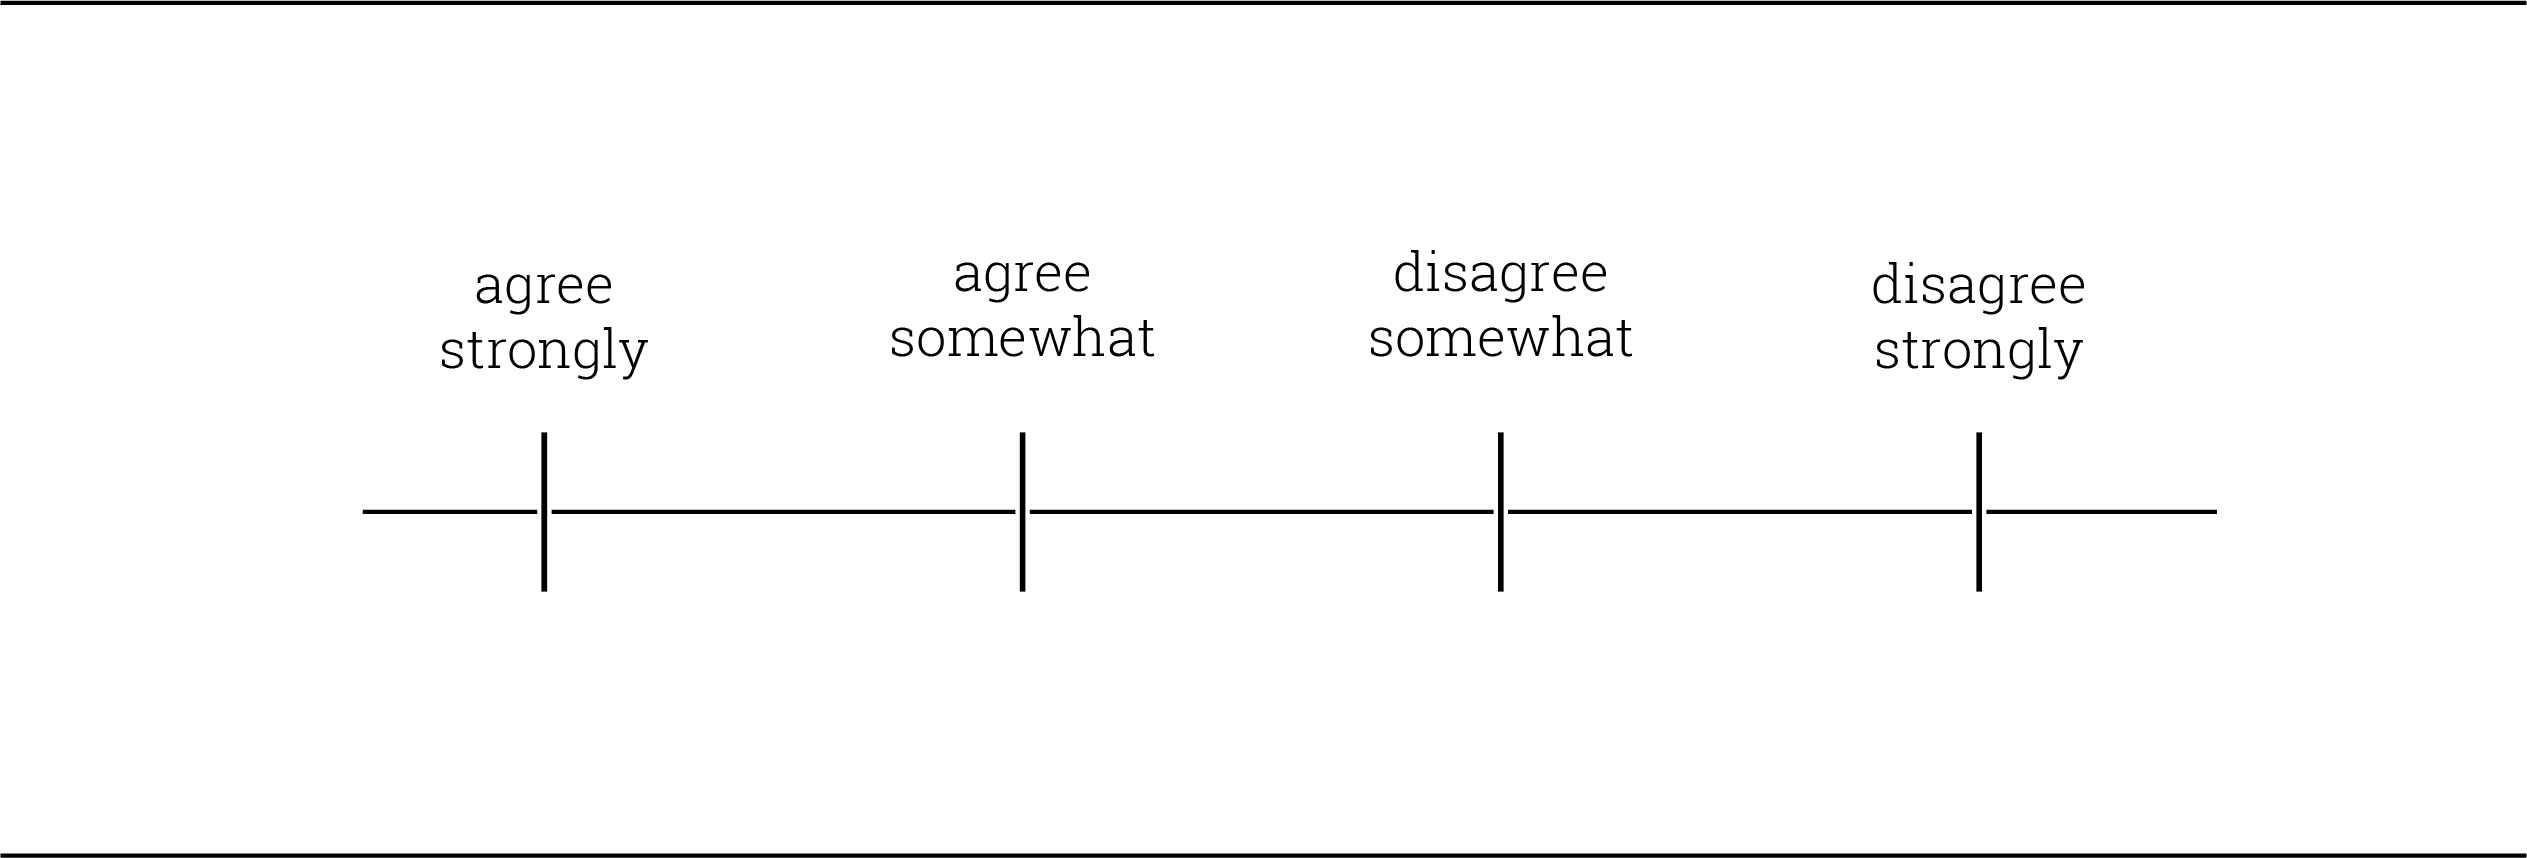
\includegraphics[width=\textwidth]{figures/FIG67fig58.png}
\caption{Four-point semantic differential Likert scale}
\label{fig:FIG67fig58}
\end{figure}

Due to the even number of statements, the participants are forced to make a basic decision. For a clearer presentation of the results, the first and second ranks are interpreted as “agreement” and the third and fourth rank as “disagreement”. All 16~participants with integrated titles rated all statements anonymously. The following statements\footnote{It cannot be ruled out that a less positive wording of the statements would have influenced the overall agreement.} were to be rated:


\begin{enumerate}
\item I could easily read all integrated titles.
\item I received all necessary information through the integrated titles.
\item I would like to watch an entire film with integrated titles.
\item I would prefer integrated titles to traditional subtitles.
\item I could spend more time exploring the image compared to traditional titles.
\item Due to the integrated titles, I was aware of more details in the image.
\item The integrated titles did not cover important elements in the image.
\item The integrated titles distracted me less from the image compared to traditional subtitles.
\end{enumerate}

\figref{fig:FIG68} shows that more than half of the participants agreed or completely agreed with the statements. While still scoring more than 80\,\% agreement, statement 6 on improved \isi{detail perception} was agreed with the least. In addition to the statements, the participants were asked to rate their \isi{aesthetic experience} (“How would you rank your \isi{overall aesthetic experience} with the integrated titles?”).

\begin{figure}
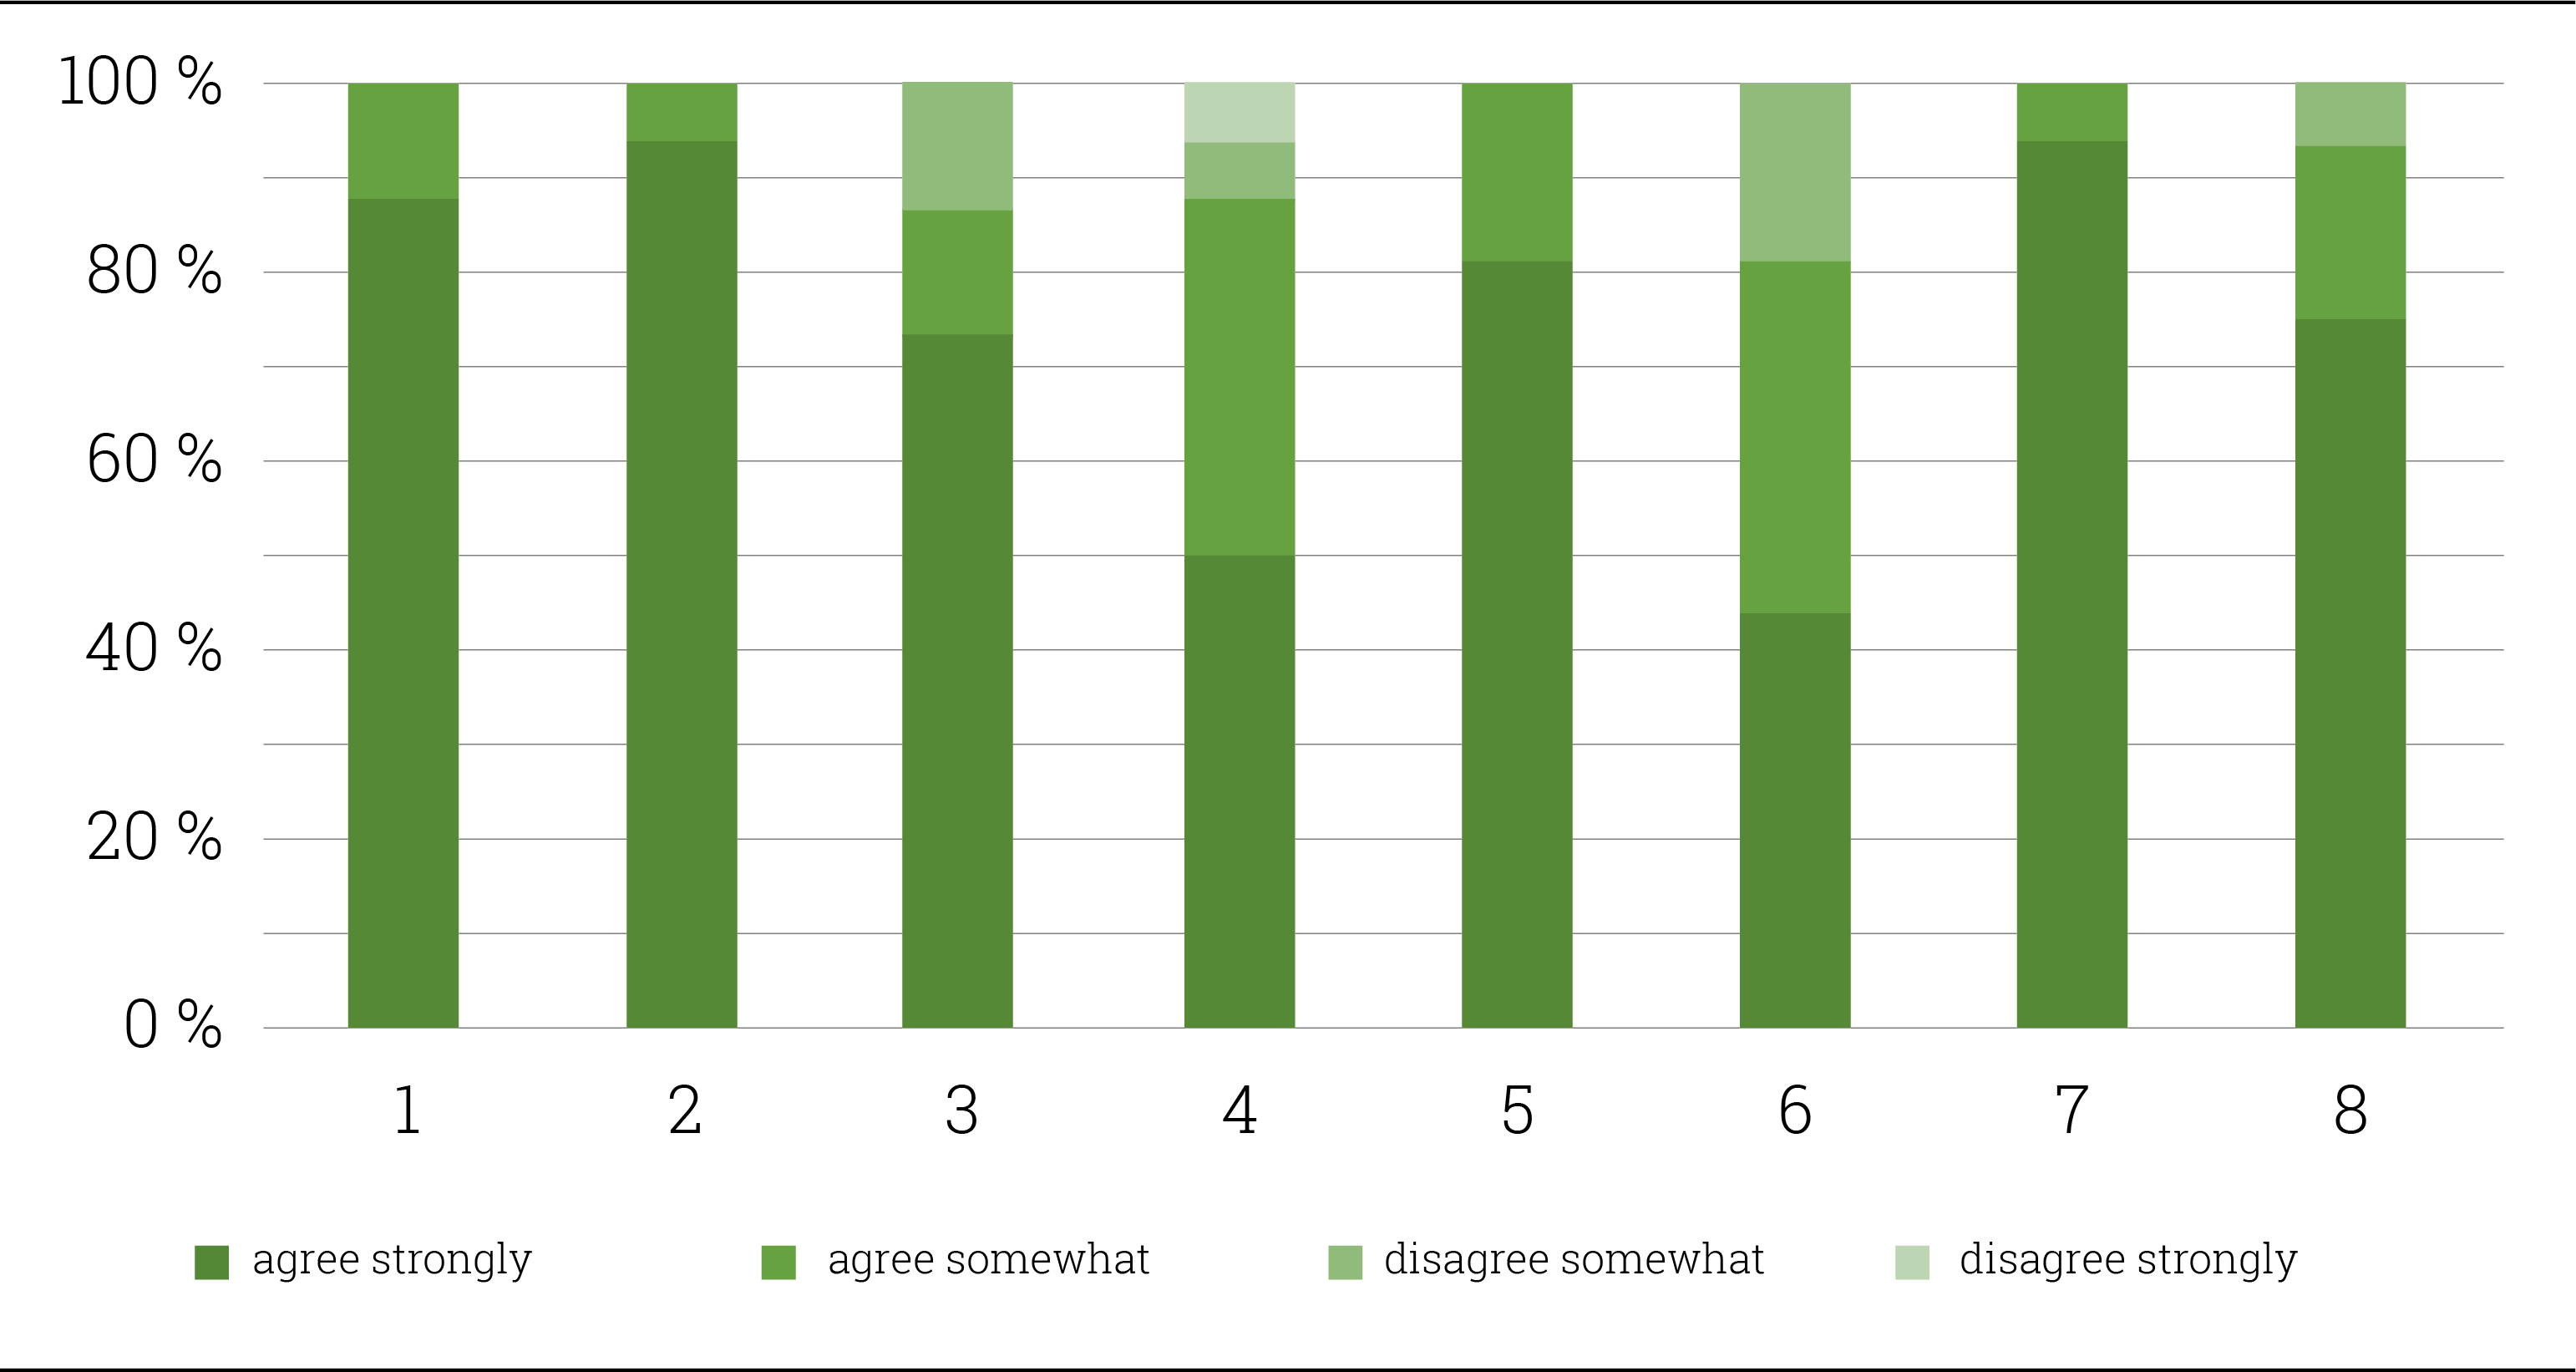
\includegraphics[width=\textwidth]{figures/FIG68chart10.png}
\caption{Agreement of the participants towards the statements}
\label{fig:FIG68}
\end{figure}

\newpage 
Concerning the fifth hypothesis on the higher \isi{information intake} (\textit{“The IT participants experience a higher \isi{information intake}.”}), two groups of the statements should be considered. The first group of statements shows that the integrated titles did not, from the participant’s point of view, decrease the \isi{information intake} (statements 1, 2, and 7), the second group indicates easier or possibly increased information extraction (statements 5 and 6). \tabref{tab:TAB15} gives a more detailed overview of these statements and shows that, except for the statement on participants being able to perceive more details, participants agreed strongly, confirming the hypothesis. Even though the cluster analysis in the previous chapter indicates that the IT participants exhibited a focus closer to the \isi{natural focus} of the English native speakers and therefore being more likely to perceive more relevant details in the image, the participants did not have this impression and accordingly rated this statement less enthusiastically.

\begin{table}
\begin{tabularx}{\textwidth}{>{\raggedright}p{39mm}SSSSS}
\lsptoprule
 \bfseries Statement &  Agree strongly &  Agree somewhat &  Disagree somewhat &  Disagree strongly\\
 \midrule
1: could read all titles & 14 & 2 & - & -\\
\tablevspace
2: all necessary information received & 15 & 1 & - & -\\
\tablevspace
5: more time for \isi{image exploration} & 13 & 3 & - & -\\
\tablevspace
6: more details perceived & 7 & 6 & 3 & -\\
\tablevspace
8: no coverage of relevant areas & 15 & 1 & - & -\\
\lspbottomrule
\end{tabularx}
\caption{Agreement to statements indicating a higher information intake}
\label{tab:TAB15}
\end{table}

\largerpage
Additionally, the participants were asked whether they generally prefer subtitling (8~participants) or \isi{dubbing} (8~participants). Those who chose \isi{dubbing} were asked to rate how likely they would prefer integrated titles to \isi{dubbing} (see \figref{fig:FIG69}). Half of the participants rated it rather likely and the other half rather unlikely. Combined with the fourth statement on preferring IT over TS, 87.5\,\% of the participants would prefer integrated titles over traditional subtitles and 50\,\% of those in favour of \isi{dubbing} would also switch to integrated titles if given the possibility.

\begin{figure}
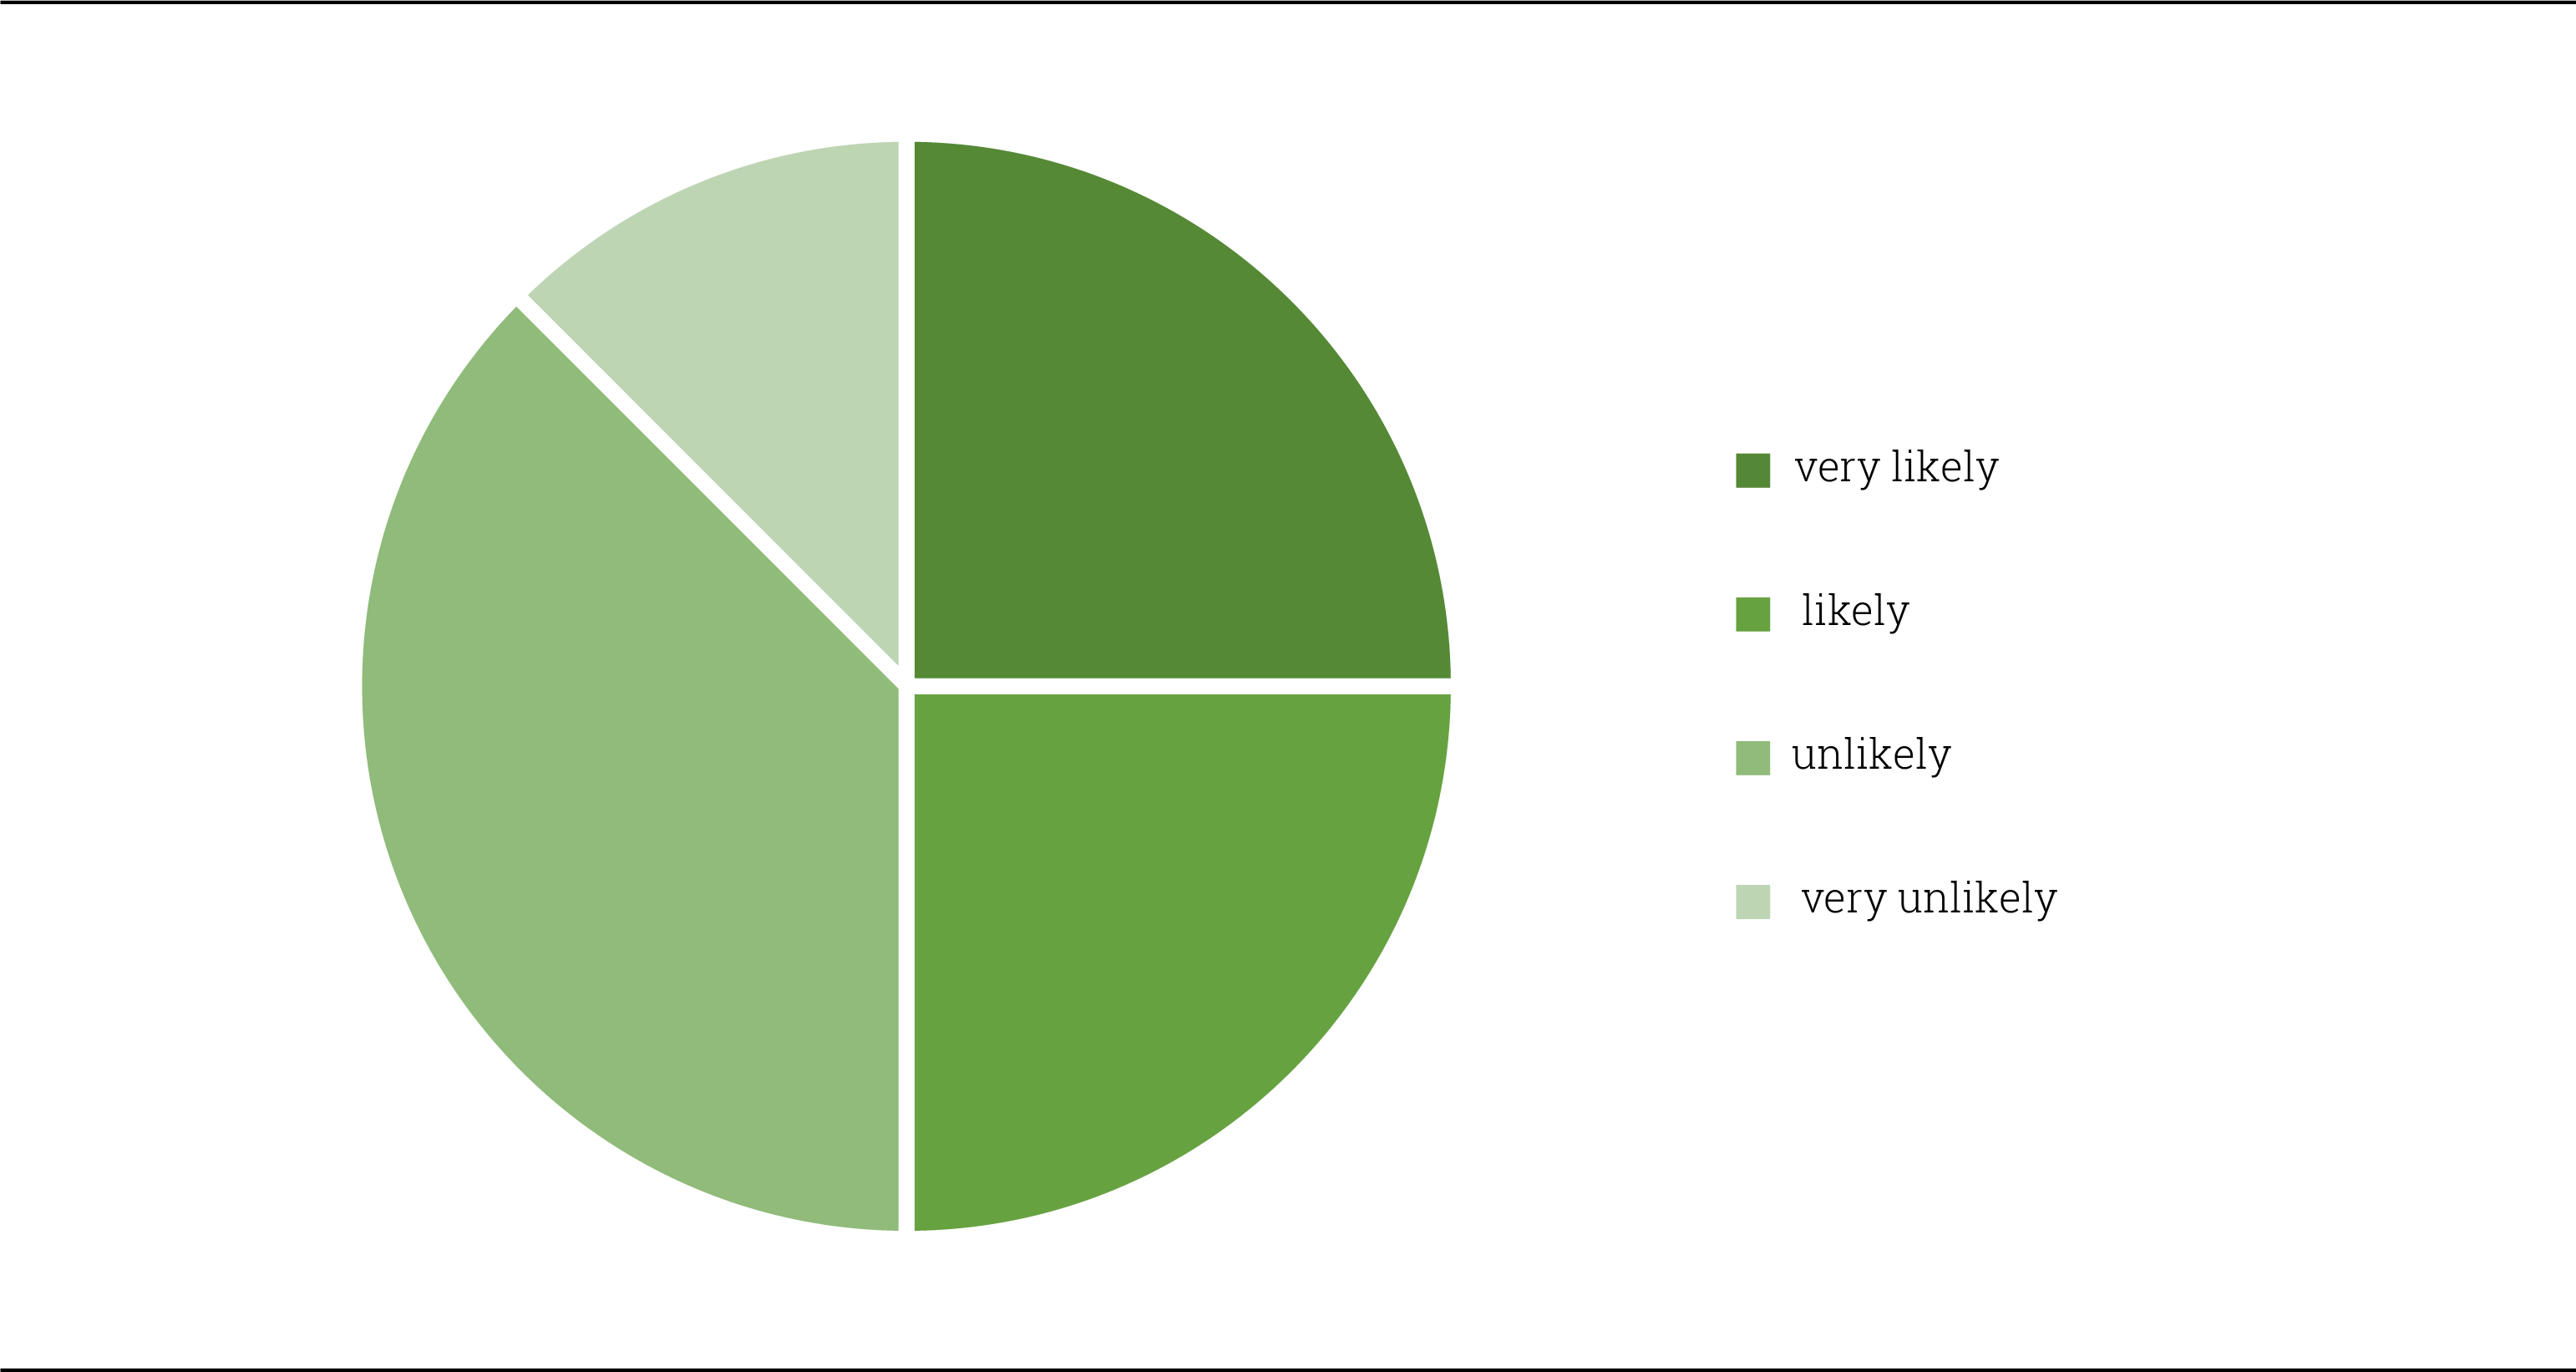
\includegraphics[width=\textwidth]{figures/FIG69chart11.png}
\caption{Likelihood of participants choosing integrated titles over dubbing}
\label{fig:FIG69}
\end{figure}


Finally, the participants were asked to rate their \isi{overall aesthetic experience} with integrated titles compared to traditional subtitles. Nine out of the 16 participants ranked it ‘very good’, seven rated it as ‘good’. None of the participants ranked it ‘satisfactory’ or ‘unsatisfactory’. This confirms the sixth hypothesis (\textit{“The integrated titles are rated as more \isi{aesthetic}.”).}


All in all, the hypotheses on the \isi{aesthetic experience} and \isi{information intake} stated an increase for both aspects for the IT participants. The evaluation of the questionnaires resulted in an overall positive rating of their \isi{aesthetic experience} by the German participants – especially when the integrated titles were compared to traditional subtitles. This positive feedback supports the hypothesis that differences in design and \isi{placement} of titles are perceived by the audience, and considerate \isi{placement} can have positive impact on the reception and information gain. Half of the participants who normally prefer \isi{dubbing}, however, did not seem to see a possible alternative in the integrated titles. Participants used to traditional subtitles on the other hand rated integrated titles as an improvement and a feasible alternative they would like to use in the future.

\section{Summary}\label{sec:8.3}

This chapter gave an overview of the results of the \isi{eye tracking} study and the questionnaire handed out to the IT participants. All \isi{eye tracking} results were significant and the questionnaire data yielded a useful insight into the subjective information gain and \isi{aesthetic experience} of the participants. As stated in the first hypothesis, the \isi{fixation duration} decreased by 14.4\,\% for integrated titles compared to traditional subtitles. At the same time, the second hypothesis was confirmed as the viewers of integrated titles spend more time exploring the image. Additionally, the IT participants exhibited a focus more similar to that of the OV participants, as stated in the third hypothesis. Here, small shortcomings of the integrated titles were easily revealed through a direct comparison to the traditional subtitles while still being overall more efficient. As presumed, the \isi{reaction time} from \isi{title display} to \isi{first fixation} in the \isi{title area} increased on average by about 25.9\,\% or 69~ms.

The analysis of the questionnaire data revealed that the majority of the participants enjoyed the integrated titles and, compared to their experiences with traditional subtitles, perceived a higher \isi{information intake} and increased \isi{entertainment value}.